% !TeX spellcheck = en_GB
\documentclass{IEEEtran}
\usepackage[utf8]{inputenc}
\usepackage{pdfpages}
\usepackage{listings}
\usepackage{booktabs}
\usepackage{float}
\usepackage{url}
\usepackage{amsmath}
\usepackage{hyperref}
\usepackage{fullpage}
\usepackage{scrextend}
\usepackage[labelfont=bf]{caption}

\graphicspath{ {img/} }

\definecolor{pblue}{rgb}{0.13,0.13,1}
\definecolor{pgreen}{rgb}{0,0.5,0}
\definecolor{pred}{rgb}{0.9,0,0}
\definecolor{pgrey}{rgb}{0.46,0.45,0.48}

% Genereal LSTListing settings
\lstdefinestyle{c} {
	language=Java,
	numbers=left,                   % where to put the line-numbers
	numberstyle=\tiny\color{gray},  % the style that is used for the line-numbers
	numbersep=8pt, 
	basicstyle=\ttfamily\footnotesize,
	showstringspaces=false,
	showspaces=false,
	showtabs=false,
	breaklines=true,
	tabsize=4,
	breakatwhitespace=true,
	commentstyle=\color{pgreen},
	keywordstyle=\color{pblue},
	stringstyle=\color{pred},
	moredelim=[is][\textcolor{pgrey}]{\%\%}{\%\%},
	frame = single, 				% For box around
	rulecolor=\color{lightgray},
	xleftmargin=\parindent,
	aboveskip=\bigskipamount
}

% Line spacing stuff
\linespread{1.25}
\setlength\parindent{0pt}
\parskip 3pt
\expandafter\def\expandafter\normalsize\expandafter{%
	\normalsize
	\setlength\abovedisplayskip{0pt}
	\setlength\belowdisplayskip{3pt}
	\setlength\abovedisplayshortskip{0pt}
	\setlength\belowdisplayshortskip{3pt}
}
%Used with scrextend package to allow fancy listing.
\addtokomafont{labelinglabel}{\sffamily}

% Title Page
\title{
	\textbf{How To Make Almost Anything:\\ Pinball Machine } \\
	Exam Project 
}

\author{
	Anders Valsted (aval@itu.dk) \\
	Elisabeth Terp Reeve (elre@itu.dk) \\
	Mathias Flintrup Jørgensen (mafj@itu.dk) \\
	Rebecca Sofie Brenøe (rebr@itu.dk) \\[6pt]
	{\small Course-code: KSHOMAA1KU }
}

\begin{document}
\maketitle
\newpage

\section{Introduction}\label{intro}
%\textcolor{red}{What is the motivation to build your device? Why is this important (at least to you)?}
This report has been written by a group of students currently studying \textit{MSc in Computer Science} on the 2\textsuperscript{nd} semester. The report is the result of a seven-week project at the IT University of Copenhagen.
It has been written in connection with the course \textit{How To Make Almost Anything} with \textit{Andres Faina}.\\\\
We decided to build a desktop sized pinball machine as our final project. Our motivation for this project, apart from it being fun, was that work was easily distributed, since a pinball machine consists of several subcomponents and obstacles. Every subcomponents (popbumpers, flippers, switches) are independent of each other and offer different challenges in regards to electronics, mechanics, software and materials. Furthermore the scope of the project was easy to adjust due to its component divided nature.
\section{Background}\label{background}
Several examples of similiar desktop sized pinball machines exist. Apart from a few toys, most of the inspiration came from other enthusiasts who have constructed these machines themselves.
One throughouly explained example is by \textit{Element 14 Presents} on YouTube \cite{presents_2017}. Other videos used for inspiration includes \textit{Arduino Pinball Machine - 3d Printing \& Lasercutting} by Fluxwood \cite{fluxwood_2018}, \textit{Arduino Pinball - Target} by Functional Design\cite{functionaldesign_2017} and \textit{DIY Tabletop Pinball Machine - Making the cabinet \& decals} by The Practical Engineer \cite{engineer_2018}.
Although much of the bodywork and dimensions on the playfield came from reference images of full sized pinball machines - an example of one of those can be seen in figure \ref{fig:playfield_example}.

\begin{figure}
	\centering
	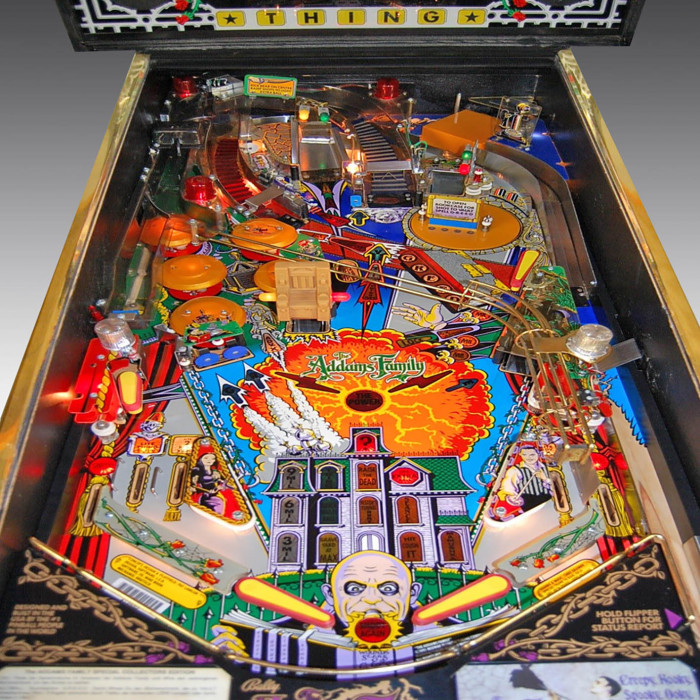
\includegraphics[scale=0.3]{img/example_playfield}
	\caption{Reference image of full sized pinball machine\cite{reference_picture}.}
	\label{fig:playfield_example}
\end{figure}
\section{Requirements}\label{requirements}
%What are the requirements or specifications? What are the capabilities that your device should have?
We were given two overall requirements for our project; the first was that the project had to contain electronics, mechanics and low level programming. The second requirement was that it had to be safe. Based on these requirements we decided on a minimum scope for our project that would make our pinball machine playable. Our minimum scope ended up including the following components:
\begin{itemize}
    \item Flippers (in the form of solenoids)
    \item Pop bumpers (in the form of solenoids)
    \item Targets with sensors (in the form of switches)
    \item A point system based on input from the different components/sensors 
    \item Display (to visualise the score)
\end{itemize}

We however ended up being ahead of time and we decided to expand the scope with the following components. We added the following components in order to make the game-play more exciting and challenging:
\begin{itemize}
    \item Dividers at the top of the board (in the form of IR sensors)
    \item Visual outputs (in the form of LEDs and RGB LED strips)
    \item Mechanism to launch ball
    \item Mechanism to return ball to launch place including registration of a lost ball (IR sensor)
    \item Ramp and decorations
\end{itemize}


\section{Description}\label{description}
%How does your device work? Describe in as much detail as you can fit into the report. It should contain three subsections: Mechanics, Electronics and Software/Firmware. Describe also what alternatives you analyzed for the different parts of your device. Why did you select the alternative that you finally used?
In the following we describe the different components of our pinball machine. In each section we describe the mechanics and electronics according to a given component. In the end of the section we describe our software implementation and how each component is wired up. 

\subsection{Flippers}
\subsubsection{Process and design}
The flippers are essentially the backbone of the machine. They are responsible for launching the ball onto the playfield. Our design closely resembles full sized pinball machines, using a linear solenoid and a lever to move the flippers.
Small tweaks during the design process improved performance, such as adjusting the length and position of the main lever and using a ball bearing for lessening friction.
\subsubsection{Final Assembly}
The flipper consists of a bracket which holds the solenoid. Then the solenoid is attached via clip and lever, to the main axis of the flipper. The flipper is inserted into a ball bearing, fixed within a bracket for the playfield. Please see figure \ref{fig:flipperassembly} for an exploded view.
\begin{figure*}
	\centering
	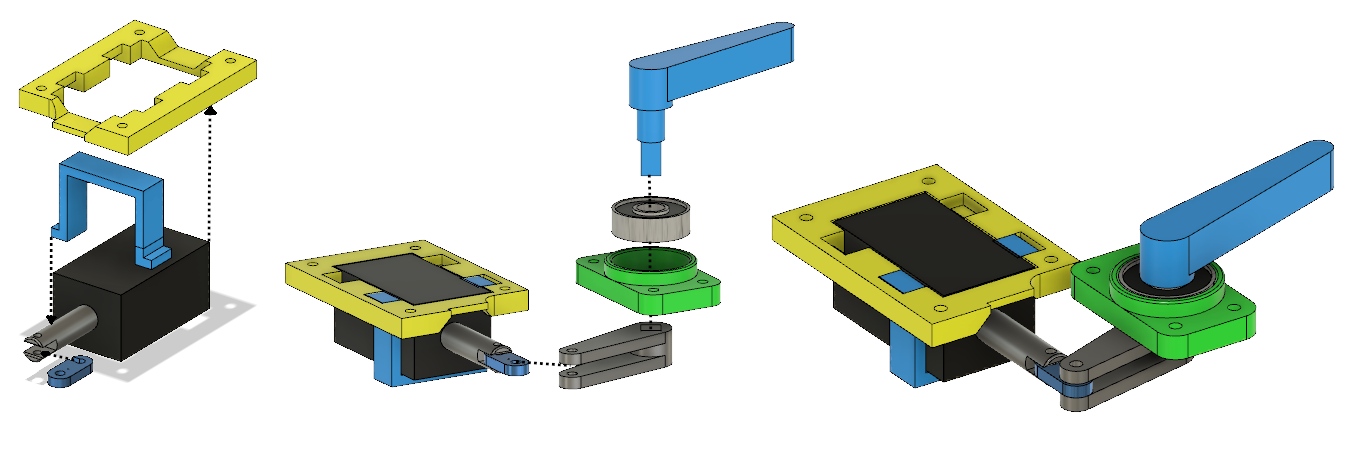
\includegraphics[width=\textwidth]{img/FlipperAssembly}
	\caption{Flipper assembly}
	\label{fig:flipperassembly}
\end{figure*}

\subsection{Pop Bumpers}
\subsubsection{Process and design}
Our first design for the pop bumpers was inspired by full sized pinball machines. It uses a linear solenoid for pulling a concave object, which when colliding with the ball, pushes it away. Most important is the detection mechanism, which uses a small plate that closes a circuit when pushed/moved. Examples of this can be seen in a video by Asker on YouTube \cite{asker_2017}. Although early tests showed that the plate was too complicated to work reliable.
Although as we improved the flipper mechanism, suddenly we had power to launch a steel ball. This meant that we could switch the pop bumpers to detect a circuit closed by the steel ball. Please see figure \ref{fig:newpop} for a image of this detection. Furthermore, for a view of the pop bumper with plate, refer to the "PopBumperWithSpoon" assembly in the "Pop Bumper" folder within the submitted Fusion 360 project.
\begin{figure}[H]
	\centering
	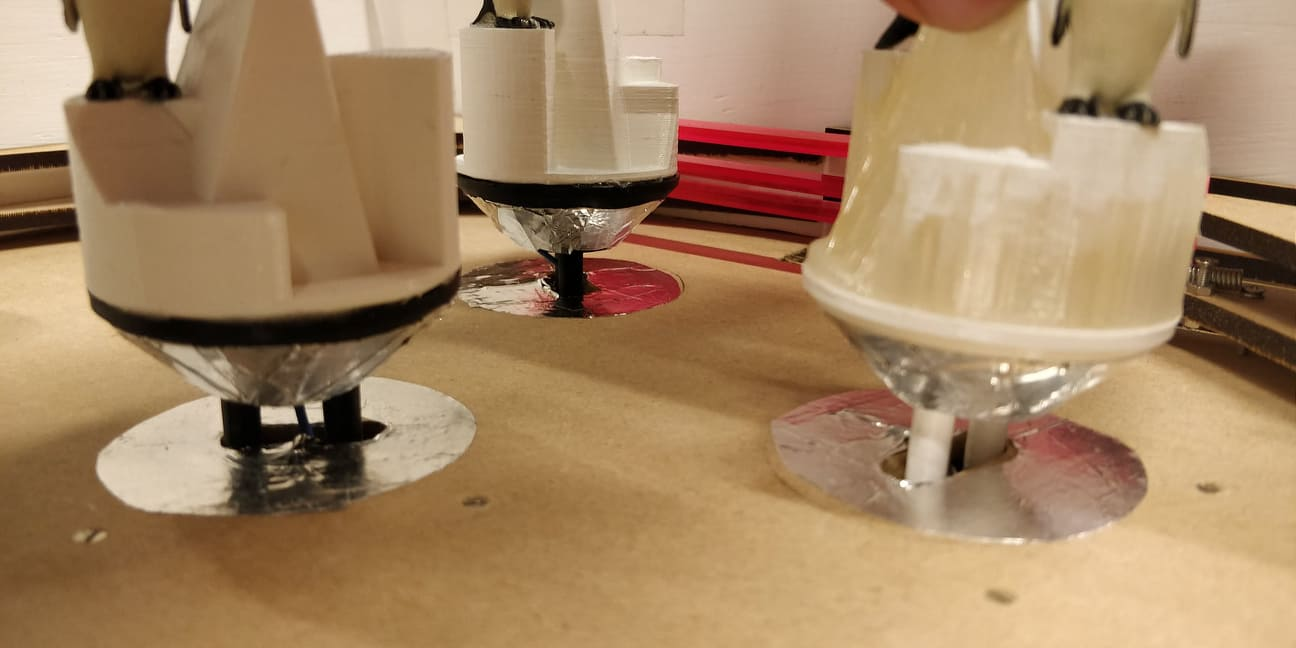
\includegraphics[scale=0.15]{img/new_bumper_design}
	\caption{The Final Pop Bumper Design}
	\label{fig:newpop}
\end{figure}

\subsubsection{Final Assembly}
The final pop bumper assembly is made up by a laser cut bracket which holds and limits the solenoid. The rest of the build is 3D printed, which includes a small bracket for the solenoid and a the hammer which pushes the ball away. Please see figure \ref{fig:bumperassembly} for an exploded view. Furthermore see Appendix \ref{appendix:cuts} for a overview of the cuts.
\begin{figure*}[h!]
	\centering
	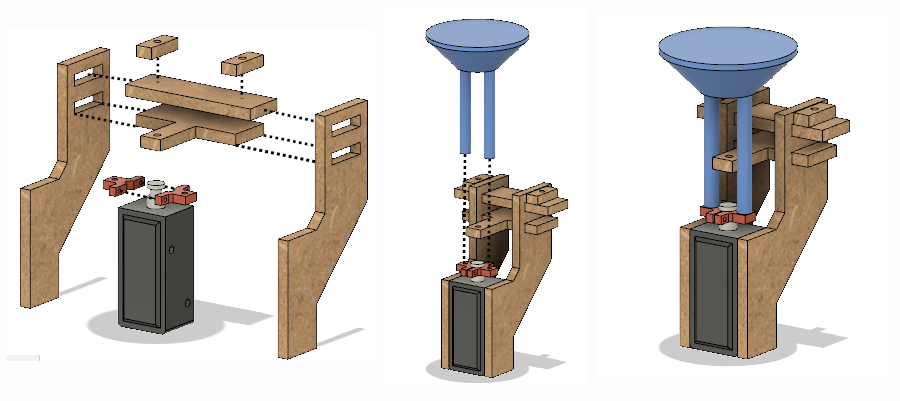
\includegraphics[width=\textwidth]{img/BumperAssembly}
	\caption{Pop Bumper Assembly}
	\label{fig:bumperassembly}
\end{figure*}

\subsection{Display}
For displaying the current score, a digital 7-segment display is used. 
It is milled into the backplate of the outer shell and encapsulated in a protective 3D-printed shell. 
Writing to the display is handled with a community Arduino library (\verb|DigitLedDisplay.h|) that talks to the  onboard MAX7219 chip. 

\subsection{Target switches}
\subsubsection{Process and design}
Switches are the main mechanism for our \textit{targets}. We found inspiration for the design of the targets in a YouTube video by \textit{Functional Design}\cite{functionaldesign_2017}. The concept builds on having a holder for a switch and a flap which is connected loosely to this holder such that it can be pushed in and activate the switch when the ball hits it. In order to visualise a hit we connected two LEDs to each holder, this means that whenever a switch is hit its associated LEDs will be turned on.

\subsubsection{Final Assembly}
The final target is modelled in Autodesk Fusion 360 and 3D printed afterwards. A target is composed of two switches, two holders, four LEDs, two flaps, and a 3D printed housing - the exploded view can be seen in figure \ref{fig:switchassembly}. We decided on having a target placed in each side of the board. The two targets share a board for their circuit which is then connected to the Arduino. When a switch is hit its associated LEDs are turned on and points are added to the total score. If a switch gets hit by the ball while the other switch on the target is turned on, all LEDs flashes for a short while and a bonus will be added to the score. 
\begin{figure*}
	\centering
	\includegraphics[width=\textwidth]{img/SwitchAssembly.png}
	\caption{Target Switch Assembly}
	\label{fig:switchassembly}
\end{figure*}

\subsection{Dividers and sensors}
\subsubsection{Process and design}
We wanted to add some mechanics to the top part of our board and we decided on having some \textit{dividers}, which should function as small walls. In order to register the ball we chose to add IR sensors in between these walls. The idea of the design of the walls is based on the fact that it had to hide a LED and a screw from the IR sensor.  

\subsubsection{Final Assembly}
Four 3D printed walls divide the top part of our board and three IR sensors are placed in each of the passages between these walls. Each wall contains an LED, and when a sensor registers the ball it will turn on the LED in the wall closest to it and points are added to the total score. If all three sensors are turned on at the same time, all LEDs will flash for a while and then turn off, also a bonus is added to the total score.
The sensors and the four LEDs share a board for their circuit and each component is connected to the Arduino. 

\subsection{Ball return mechanism}
The ball return mechanism consists of a slide going from a spring loaded pulley to a self-closing door on the playfield.

\subsubsection{Final assembly}
The parts are all laser cut using 4mm material of choice and then assembled using glue or screws. Exploded view is shown in figure \ref{fig:slideassembly}. Furthermore see Appendix \ref{appendix:cuts} for a overview of the cuts.
\begin{figure*}
	\centering
	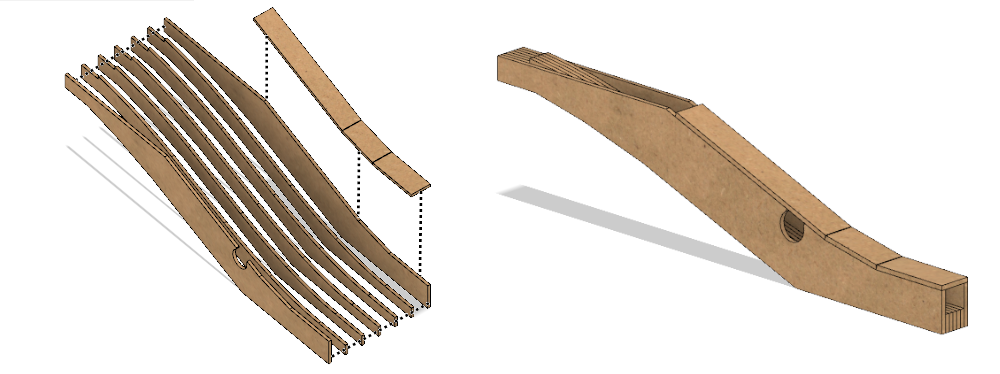
\includegraphics[width=\textwidth]{img/SlideMechanismAssembly}
	\caption{Slide mechanism assembly}
	\label{fig:slideassembly}
\end{figure*}

\subsection{The playfield}
The playfield of the machine is all bodywork on top, including the obstacles, ball return mechanism and bounding walls. All stationary walls were laser cut and fixed either by screws or brackets. The placement of the obstacles and point giving object can be changed and is not predetermined. Here, we give an example of how to place these.

\subsubsection{Final assembly of bodywork}
Every wall piece is laser cut from a 4mm material of choice. Then they are mounted with screws and spacers. Please see figure \ref{fig:bodyassembly} for an exploded view. Furthermore see Appendix \ref{appendix:cuts} for a overview of the cuts.
\begin{figure*}
	\centering
	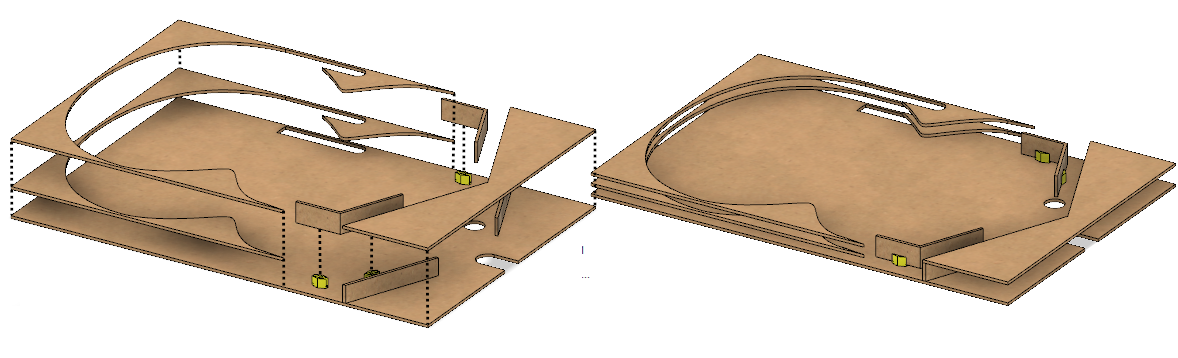
\includegraphics[width=\textwidth]{img/PlayFieldBodyAssembly}
	\caption{Playfield bodywork assembly}
	\label{fig:bodyassembly}
\end{figure*}

\subsubsection{Attaching the mechanisms to playfield}
Flippers and the ball-return mechanism both fit into the appropriate holes. All the other mechanism have appropriate holes for screws, and these can be attached whereever on	es sees fit. Please see figure \ref{fig:mechanismassembly} for an exploded view.
\begin{figure*}
	\centering
	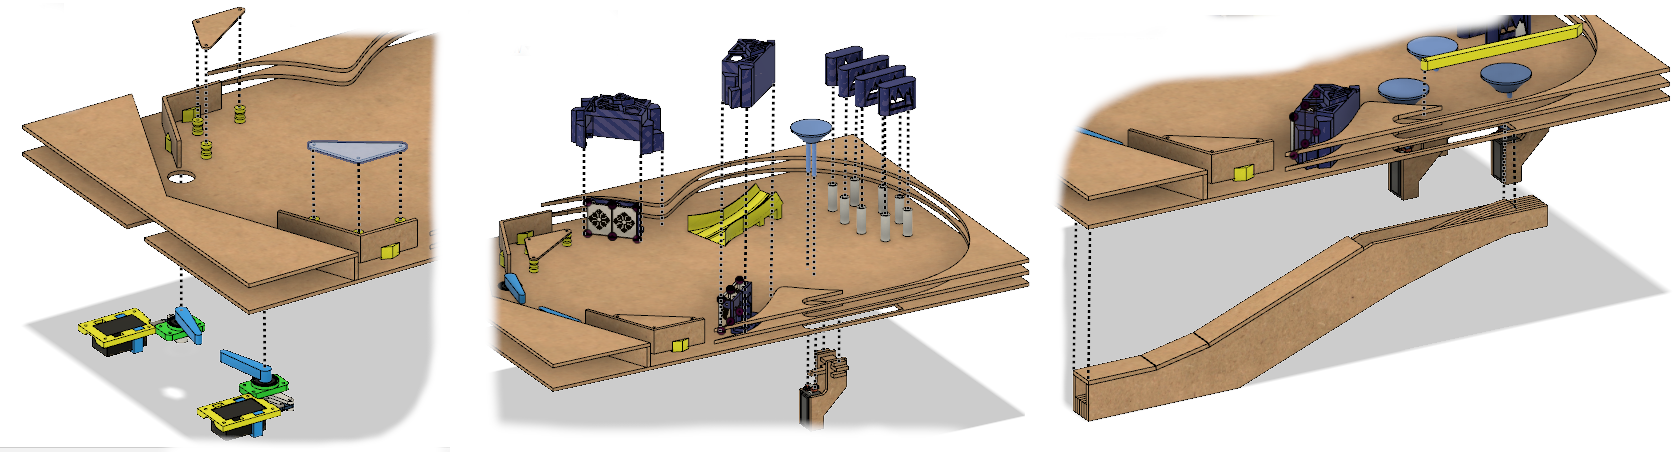
\includegraphics[width=\textwidth]{img/PlayFieldMechanismAssembly}
	\caption{Assembly for all mechanisms on playfield.}
	\label{fig:mechanismassembly}
\end{figure*}

\subsection{The Software Implementation}
The whole show is driven by an Arduino Mega, for which a wiring diagram is supplied in figure \ref{fig:wiring}.
Black wires indicate input, {\color{red} red} wires indicate output, and {\color{blue} blue} are for two-way communication. 
An more comprehensive overview of the functional blocks in the machine is given in appendix figure \ref{fig:funcdiag}

The pinball machine domain is largely event-driven, unlike the sequential nature of the Arduino. 
We had to avoid use of the delay function in order to be responsive to button/switch/IR sensor inputs at arbitrary times. 
A concurrent model, inspired by the Adafruit guide in \cite{multitasking_arduino}, was chosen as the solution. We describe this model in more detail in appendix \ref{appendix:programming model}.
\begin{figure}[h]
	\centering
	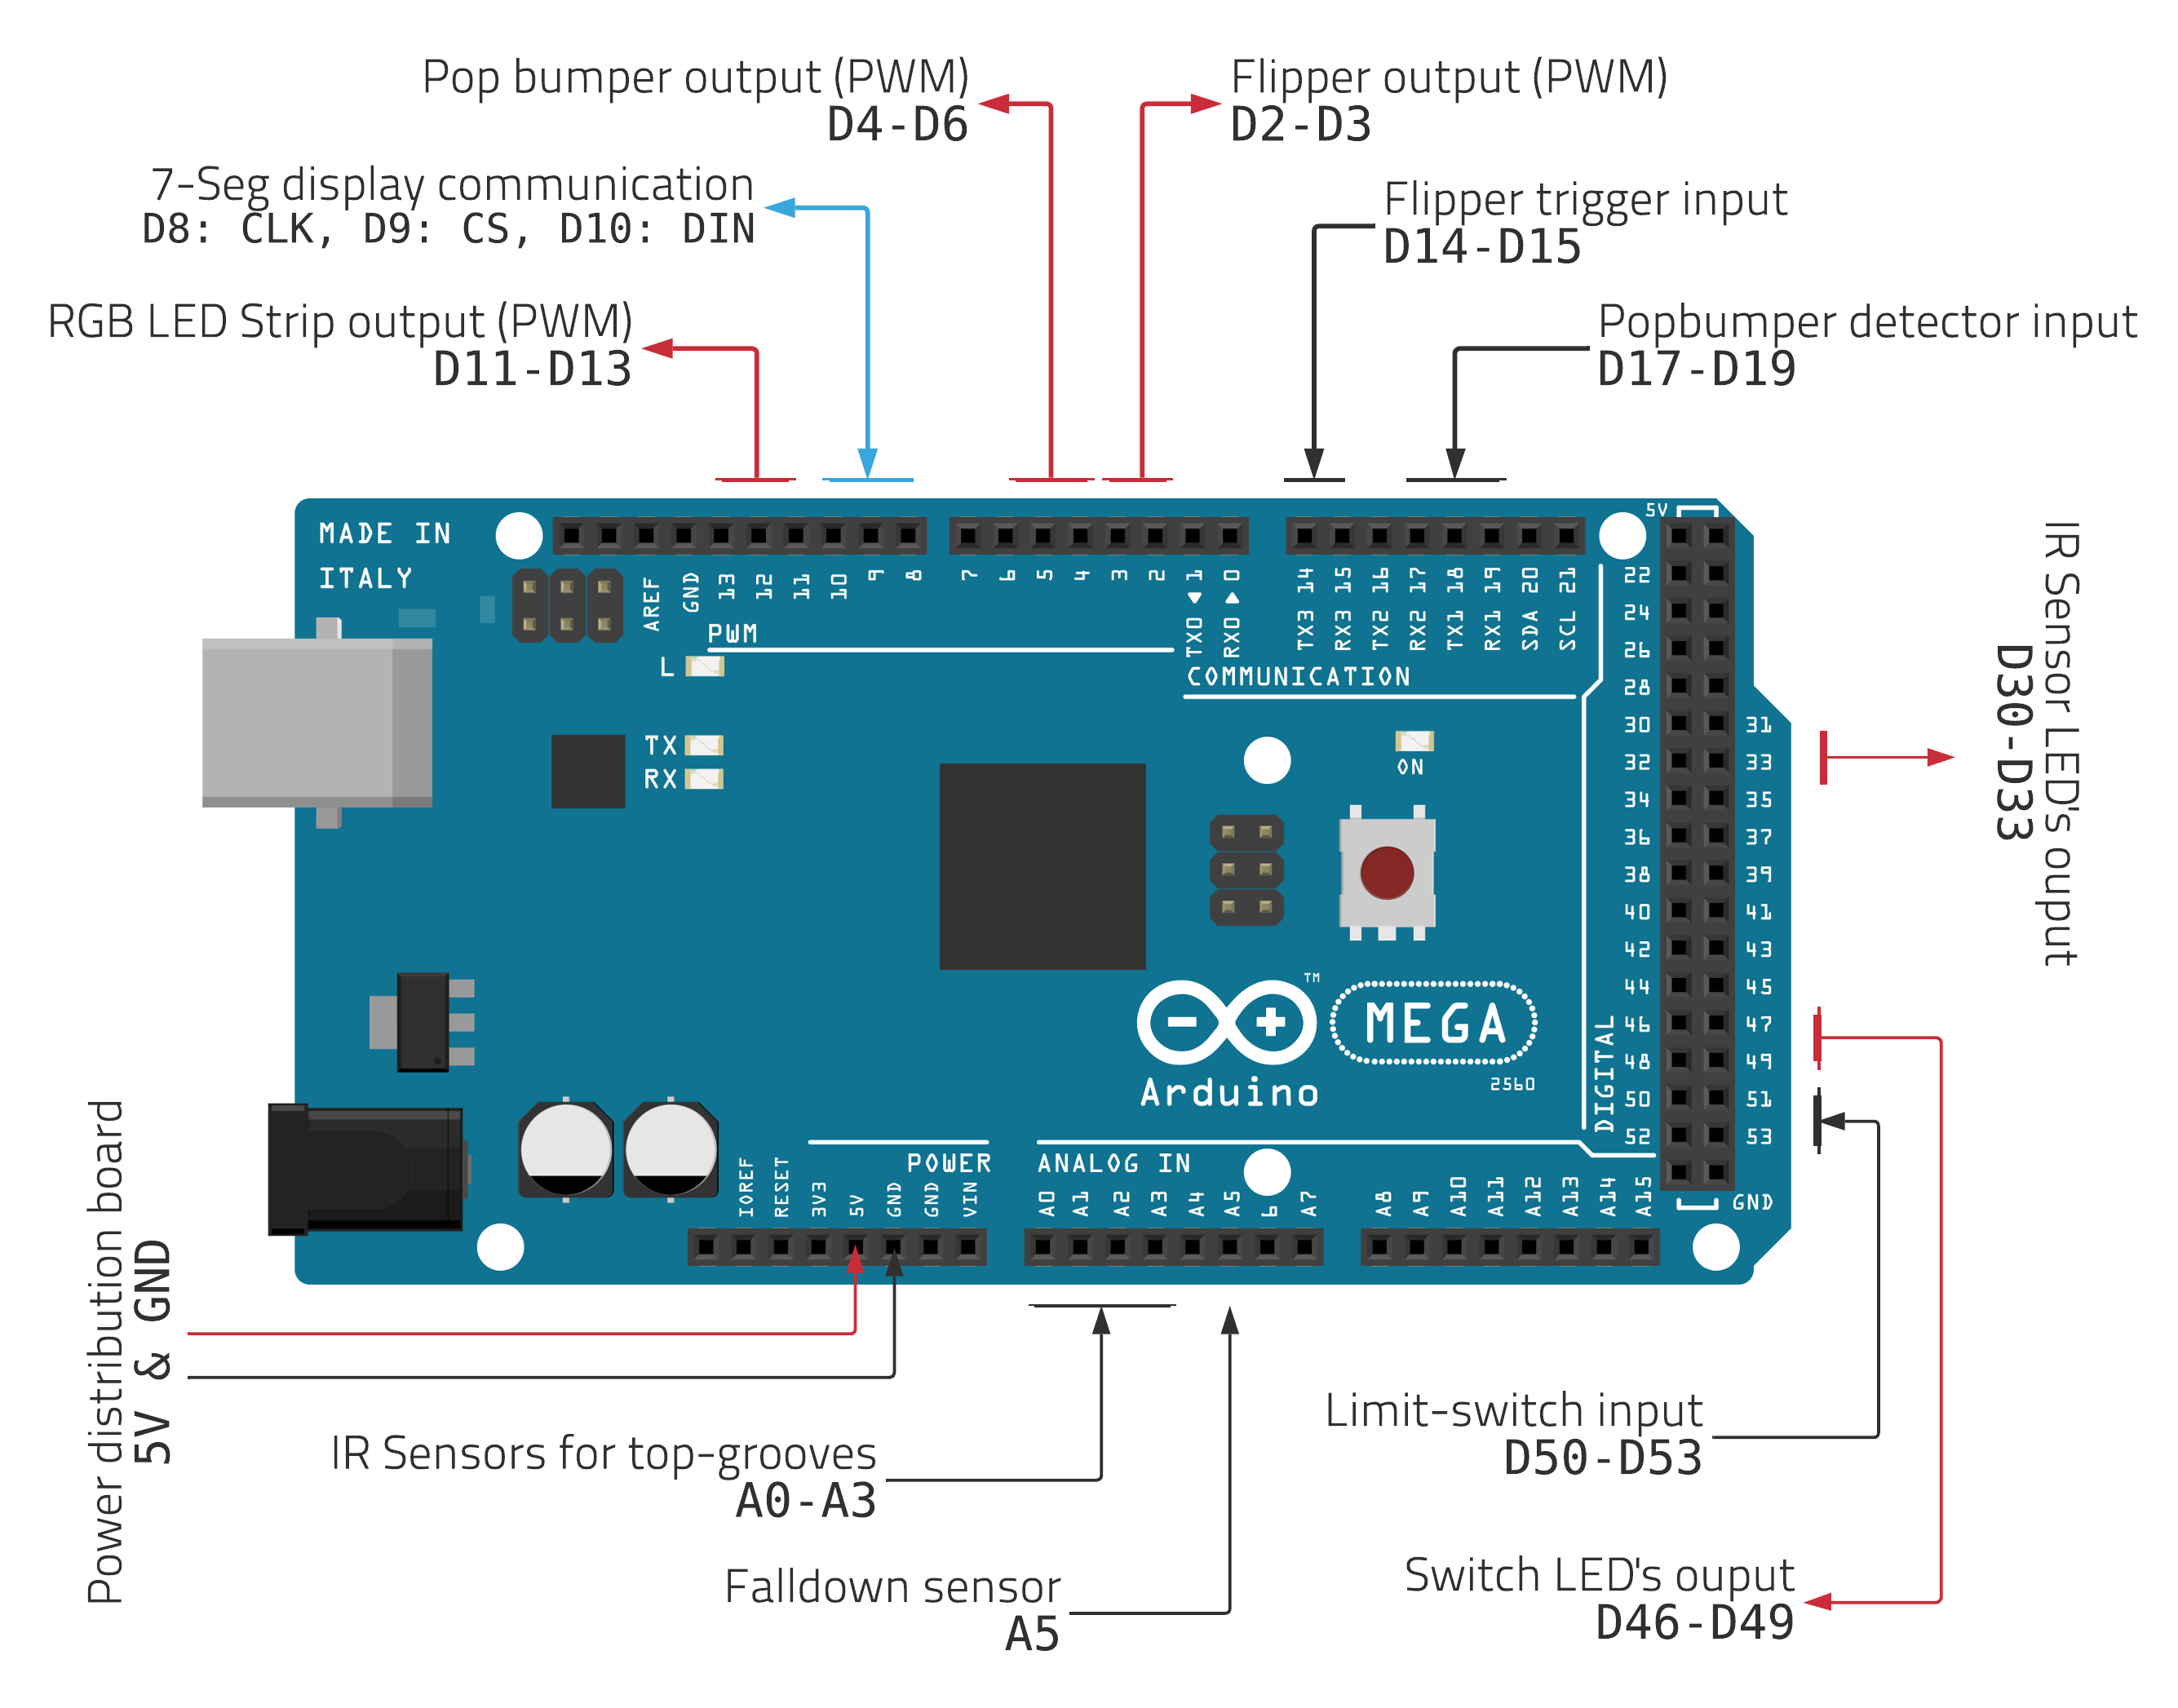
\includegraphics[width=0.46\textwidth]{wiring_diagram}
	\caption{How the Arduino Mega is wired up to the project interface boards.}
	\label{fig:wiring}
\end{figure}
\subsection{Putting it all together}
\begin{figure}[h]
	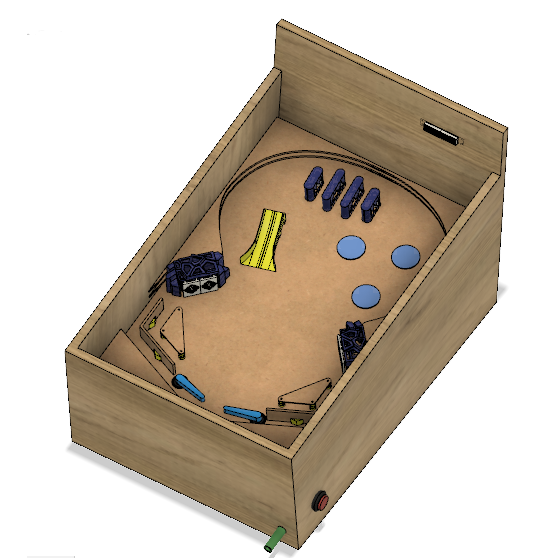
\includegraphics[width=\textwidth/2]{FinalAssembly}
	\caption{View of the final assembly 3D reference.}
	\label{fig:finalassembly}
\end{figure} 
The final playfield assembly is lowered into a plywood box with cut rails for support. Here, the segment display and spring loaded mechanism is attached. Figure \ref{fig:finalassembly} shows the final assembled version 3D reference model. This model, named FinalAssembly in Fusion 360, can be used to source the necessary dimensions of the surrounding box.



\section{Results/analysis}\label{analysis}
%Did it work properly? What kind of tests did you run to test your prototype? Could you provide some data that shows the performance of the prototype (speed, success rate, etc.)?

%Did it work probably?
\subsection{Implementation of project}
Our final end product ended up being very similar to our expected reference model. See figure \ref{fig:sbs} for a comparison of the reference model and the final implementation.
\begin{figure*}[h]
	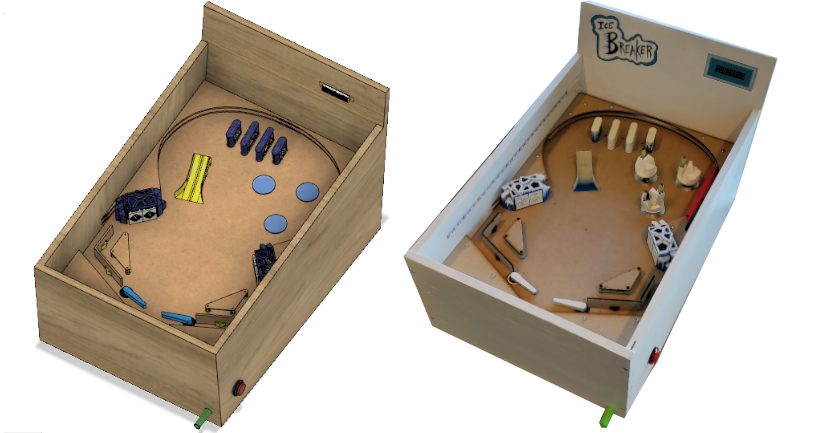
\includegraphics[width=\textwidth]{SideBySide}
	\caption{Side by side view of reference model (left) and image of final implementation (right). See Fusion 360 model named FinalAssembly for reference model.}
	\label{fig:sbs}
\end{figure*}
Individually we got every electronic mechanism/subcomponent working using an Arduino. When later combined, all the electronics software was loaded onto one Arduino Mega, which worked as expected. Please see the alongside submitted video for a presentation of the subcomponents working together on the assembled version.
\subsection{Shortcomings}
\subsubsection{Flippers}
During the final assembly, unfortunately the board used for distributing regulated power to the flippers broke. Although, as we proved during earlier tests, the layout worked as intended. For the final presentation, we did a workaround for showcasing the mechanism.
\subsubsection{Fall down mechanism}
Unfortunately the registration of a ball being lost, was de-scoped for the final presentation. We simply needed more time for tuning the sensor so that it worked reliably. Although the software for registration, counting and displaying lives are ready. 
\subsubsection{Ramp}
The ramp in the upper left corner of the playfield was originally intended to have rails for moving the ball across the playfield. Although due to time constrains, this was de-scoped. The final implementation although still has the ramp installed.
\subsection{The construction process}
\subsubsection{General}	
Since the project is made of many smaller subcomponents we had the chance to create these components independent of each other. This meant that we had the ability to test each component's mechanism, electronics and software separately before putting everything together. This way it was easier to test the project as a whole and to combine all the components to create the final prototype.\\
\subsubsection{Mechanism}
To make sure that the mechanism of a component was working, a model would first be created in Autodesk Fusion 360 and \textit{joined} together with other components if it interacted with them. Then one copy would be produced and tested. If the component worked, the rest of the components of the same type would be produced the same way, otherwise the 3D model would be configured to fit better and reproduced. This iterative process would continue until a successful component was created.\\
\subsubsection{Electronics}
Similar to the mechanisms, our electronic circuits were tested separately before expanded and soldered onto perf-board.
This was especially important, as we were dealing with multiple components that used either 5, 12 or 24 volts voltage. These were tested separately from the Arduino to avoid short circuits. We did this using buck boosts. 
\subsubsection{Software}
After we made sure the mechanisms and electronics worked for a component we added the software to it. Each component had their own Arduino-sketch class where all their own logic existed. Here we could test the code for each component and make sure that it worked as it should before declaring the component completely finished.
\\
To compensate for having all subcomponents logic on one Arduino, we had to rule out the often used "delay" method for waiting for a process. This event-driven process meant that no call was blocking. See appendix \ref{appendix:programming model} for further details about our programming model.
\\
Finally we combined all the Arduino-sketch classes into one main class.

\section{Discussion}\label{discussion}
%What are the strengths and shortcomings of your device? Did it match the requirements?  How would you improve/develop it further, if you had time? If you had to produce your device in a factory for mass production, what would you modify? 

One of the biggest strength of our pinball machine is the almost complete independence of the different components. 
Since each component is independent, it is incredible easy to change and add new components to the board. This was also part of the motivation for choosing this project, that it was easy to add new components and effects to the project .\\

If we continued working on the project we do have some things we would like to change; 

First we tried to add a sensor by the hole, where the ball is returned to launch place, to create a way for the player to lose the game. However, when we tested the sensor it became obvious that we could not get any useful readings for it, in the environment we had chosen for it. Unfortunately it was so late in the project that we did not have time to try and fix this problem. This would probably be a pretty simple fix that would improve the player experience.

It would also be preferable to add more ways for the player to get point. An easy one would be to make the ramp be part of the point system by adding an sensor or a switch.

Finally it would be nice to add a bigger display so it would be easier for the player to keep track of their lives, score and other important player information e.g. high scores.\\

If we needed to mass produce this project it would first and furthermost be a great idea simulate the game. This way we could make sure that all components could be activated, which placements are best and that the game has a good flow.

We have multiple incidents where this would have benefited us, especially regarding placement of the components. A good example of this is the ramp, which had to be moved in order for us to hit it at the right angle.

We also relied heavenly on 3D-printing for a lot of our components, which would needed to be switched out with other more efficient methods such as molding or laser-cutting. The holes in the board for screws was also added along the way manually, this should be done when the playing field is laser-cut. 

%Another thing would be to create PCBs for all the circuits now that we know the components are working and the circuits are final.

\bibliographystyle{plain}
\bibliography{biblio}
\newpage
\appendix
\subsection{Functional blocks overview}
Figure \ref{fig:funcdiag} provides an overview of the functional components making up the pinball-machine.
\begin{figure*}
	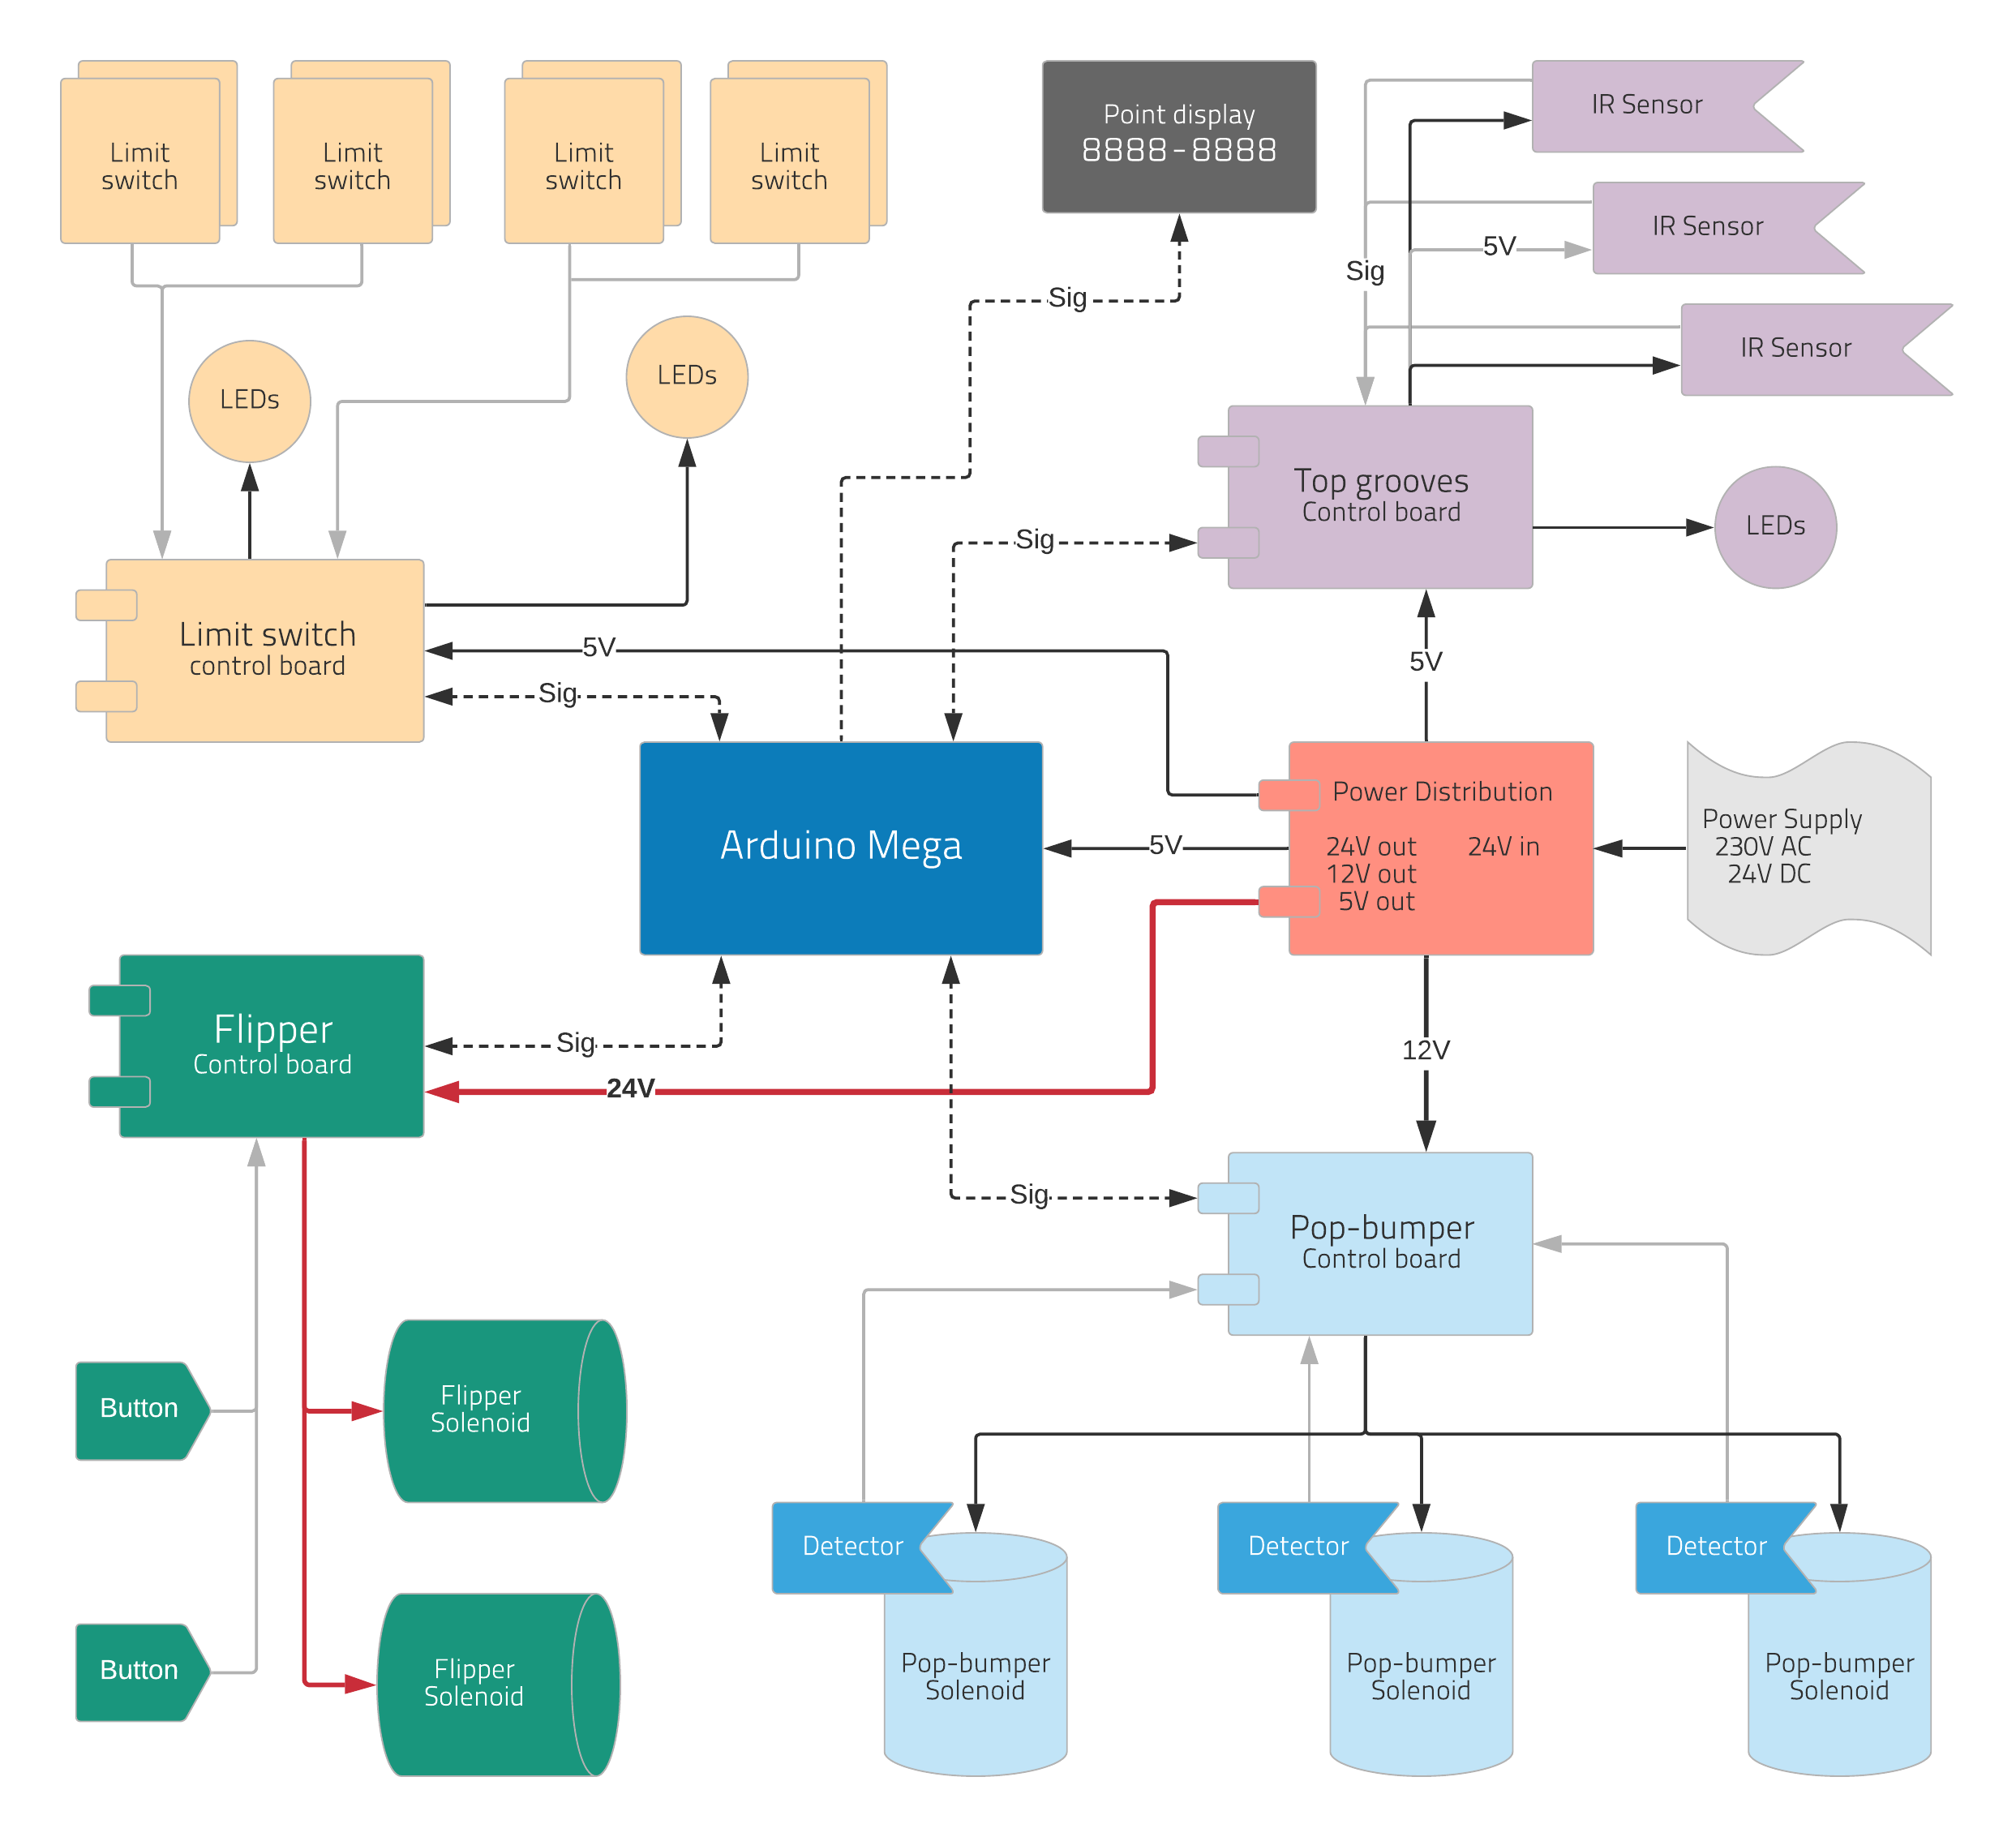
\includegraphics[width=\textwidth]{functional_diagram}
	\caption{Overview of the main electrical components in the pinball-machine.}
	\label{fig:funcdiag}
\end{figure*}

\subsection{Circuits}
Quite early in the project it became apparent that a lot of interfacing between the arduino and the individual components would be necessary. 
Thus, we split each functional component up into its own sub-circuit. 
Each sub-circuit is realized on a separate perf-board with pin-headers mounted for external interfacing (see figure \ref{fig:perfboard}). 
The idea is to abstract away power delivery and intermediary connections, such only control pins are routed to the Arduino. 
Power delivery to each board is handled by wires to a common power-distribution board. 
It consists of two XL6009 dc-dc buck-converters, down-stepping the power supply's 24V to 5V and 12V respectively (see figure \ref{fig:powboard}).

\subsection{Schematics}
In table \ref{tab:circuits} the schematics for the primary sub-circuits used in the pinball machine are summarized.

\begin{table*}[h]
	\centering
	\begin{tabular}{@{}lll@{}}
		\toprule
		Circuit & Is shown in & Description \\ \midrule
		\textbf{Flippers}       & Figure  \ref{cir:flipper}  & Reads two buttons and drives two mosFETs.                    \\ 
		\textbf{Popbumpers}     & Figure  \ref{cir:bumper}   & Reads three pieces conductive-tape and drives three mosFETs. \\
		\textbf{Dividers}       & Figure  \ref{cir:top}      & Reads three IR-sensors and controls four LEDs.               \\
		\textbf{Limit-switches} & Figure  \ref{cir:switches} & Reads four switches and controls four LEDs.                  \\
		\textbf{RGB-strip}      & Figure  \ref{cir:rgbled}   & Drives three high-current transistors.                       \\ \bottomrule
	\end{tabular}
	\caption{Circuit index.}
	\label{tab:circuits}
\end{table*}

% ================== POWER =======================
\begin{figure}[h]
	\centering
	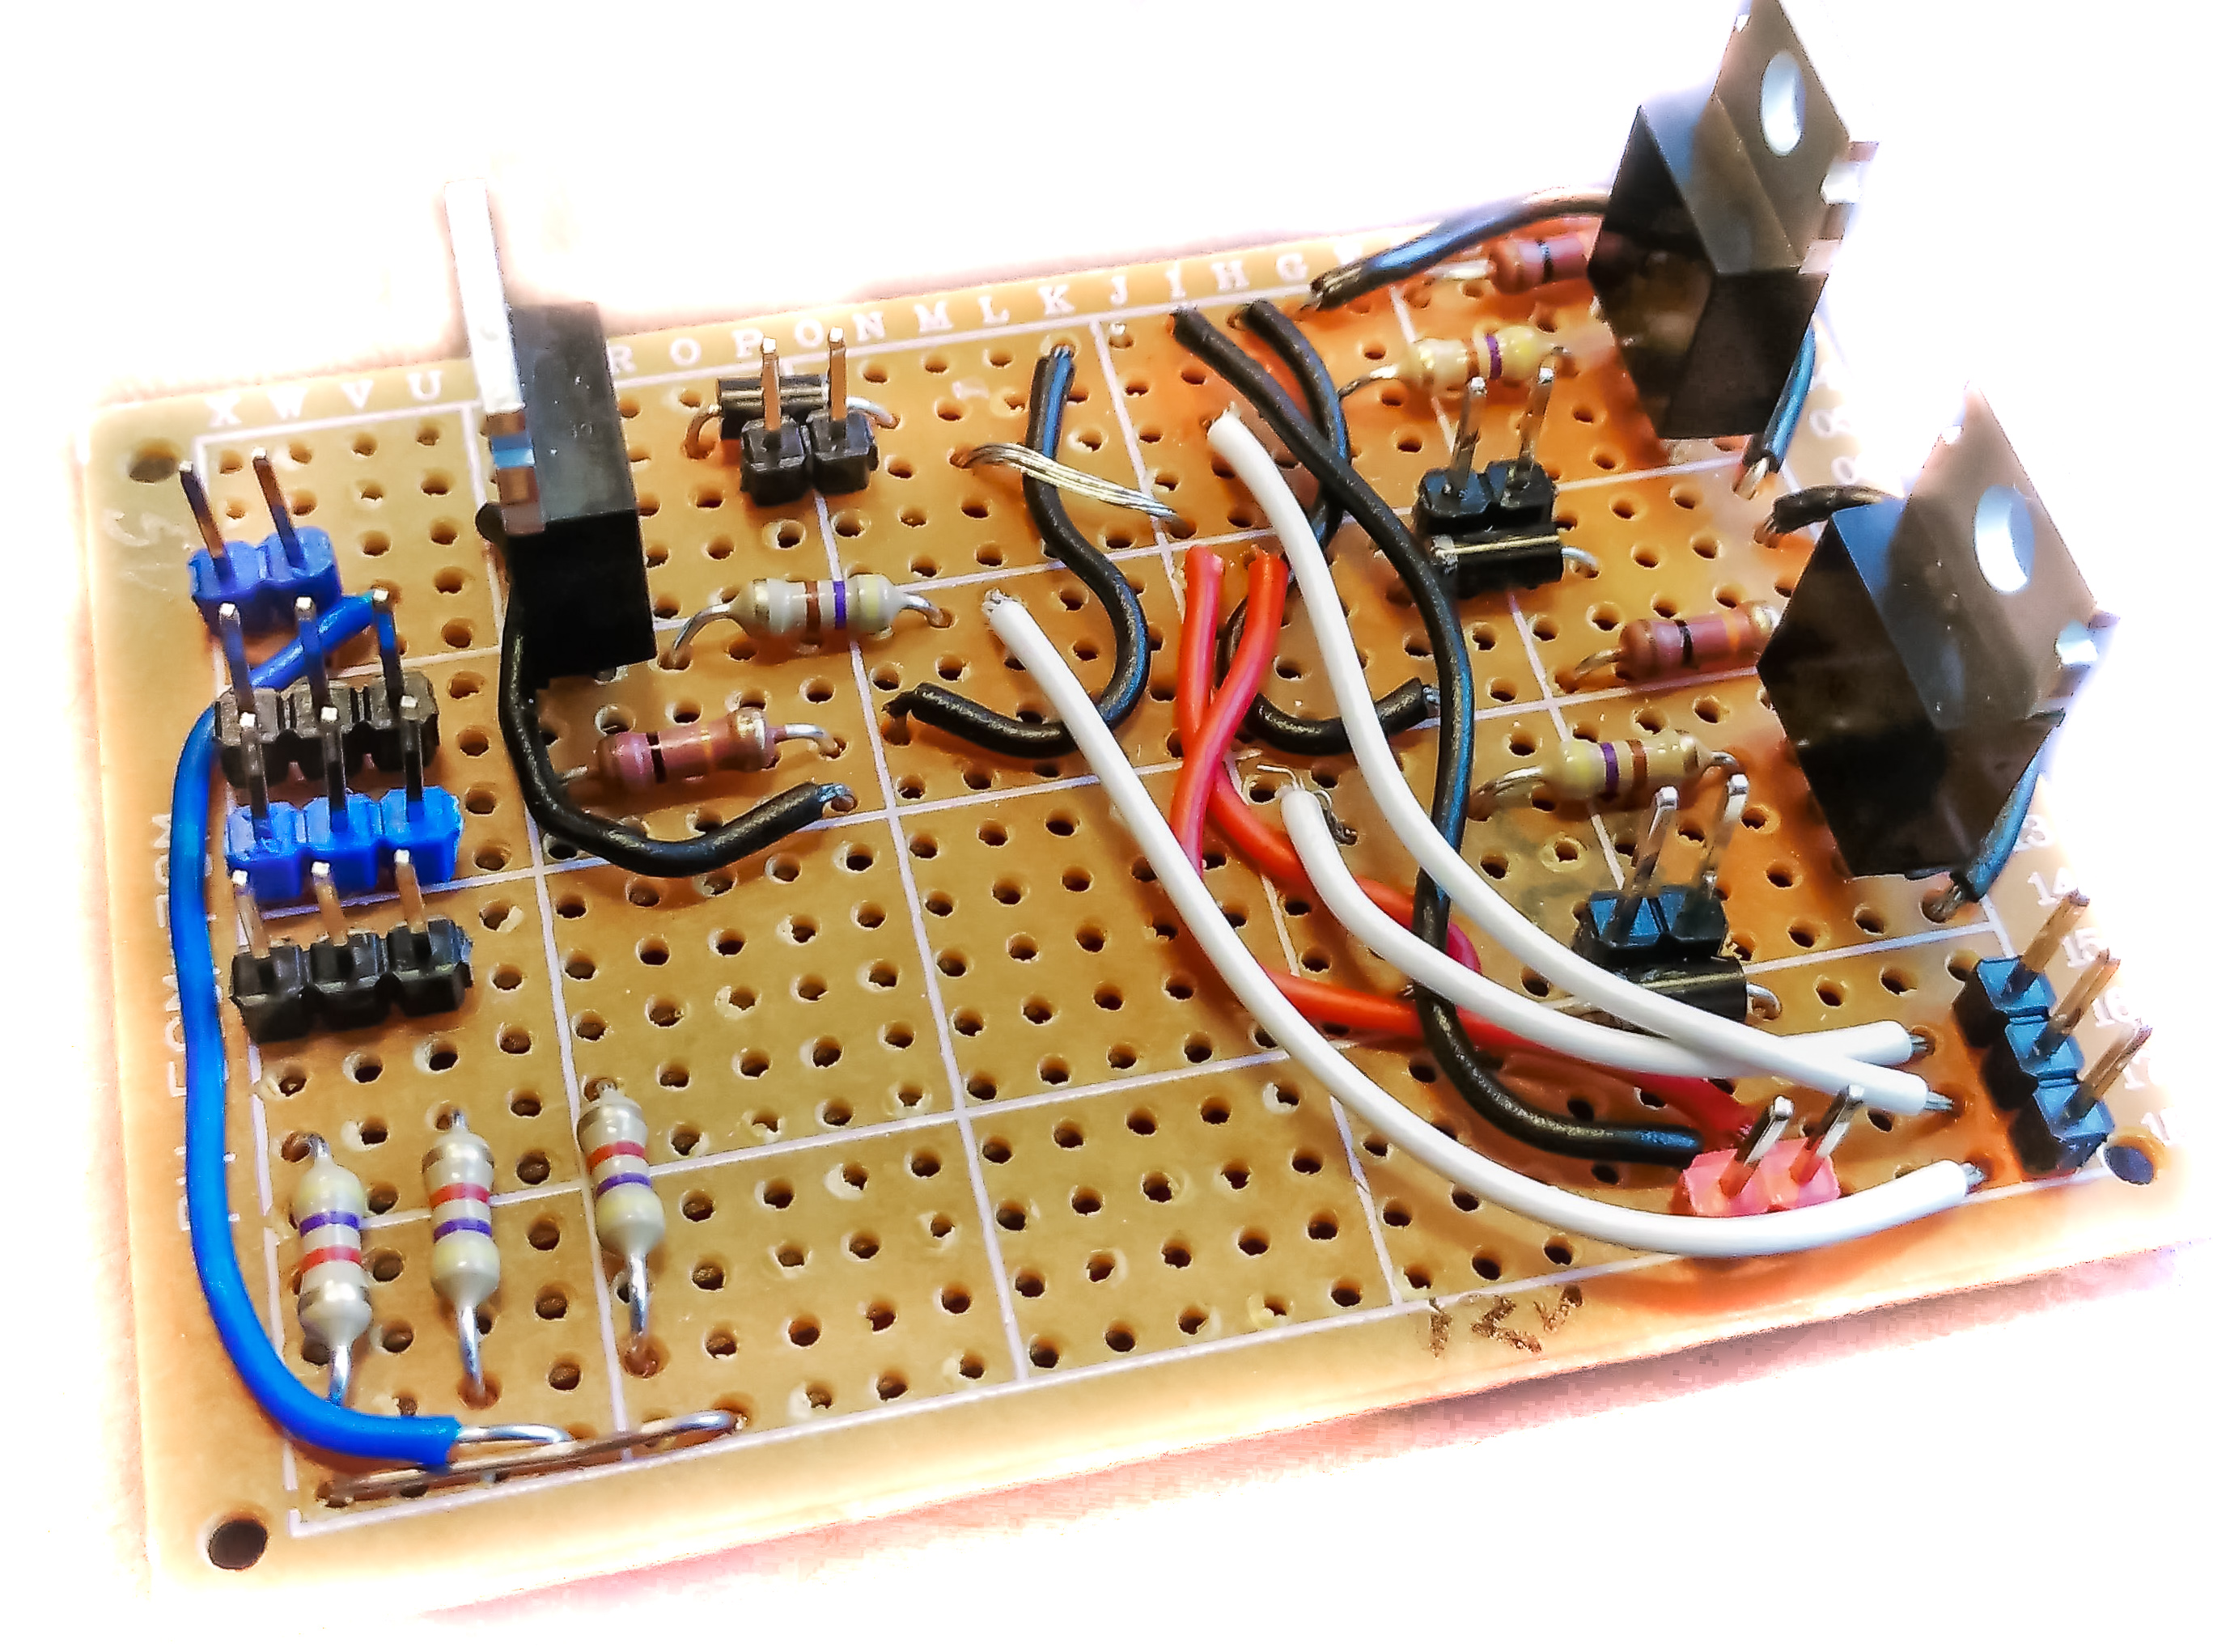
\includegraphics[width=0.42\textwidth]{popbumper_perf}
	\caption{Subcircuit board for controlling the popbumpers.}
	\label{fig:perfboard}
\end{figure}

\begin{figure}[h]
	\centering
	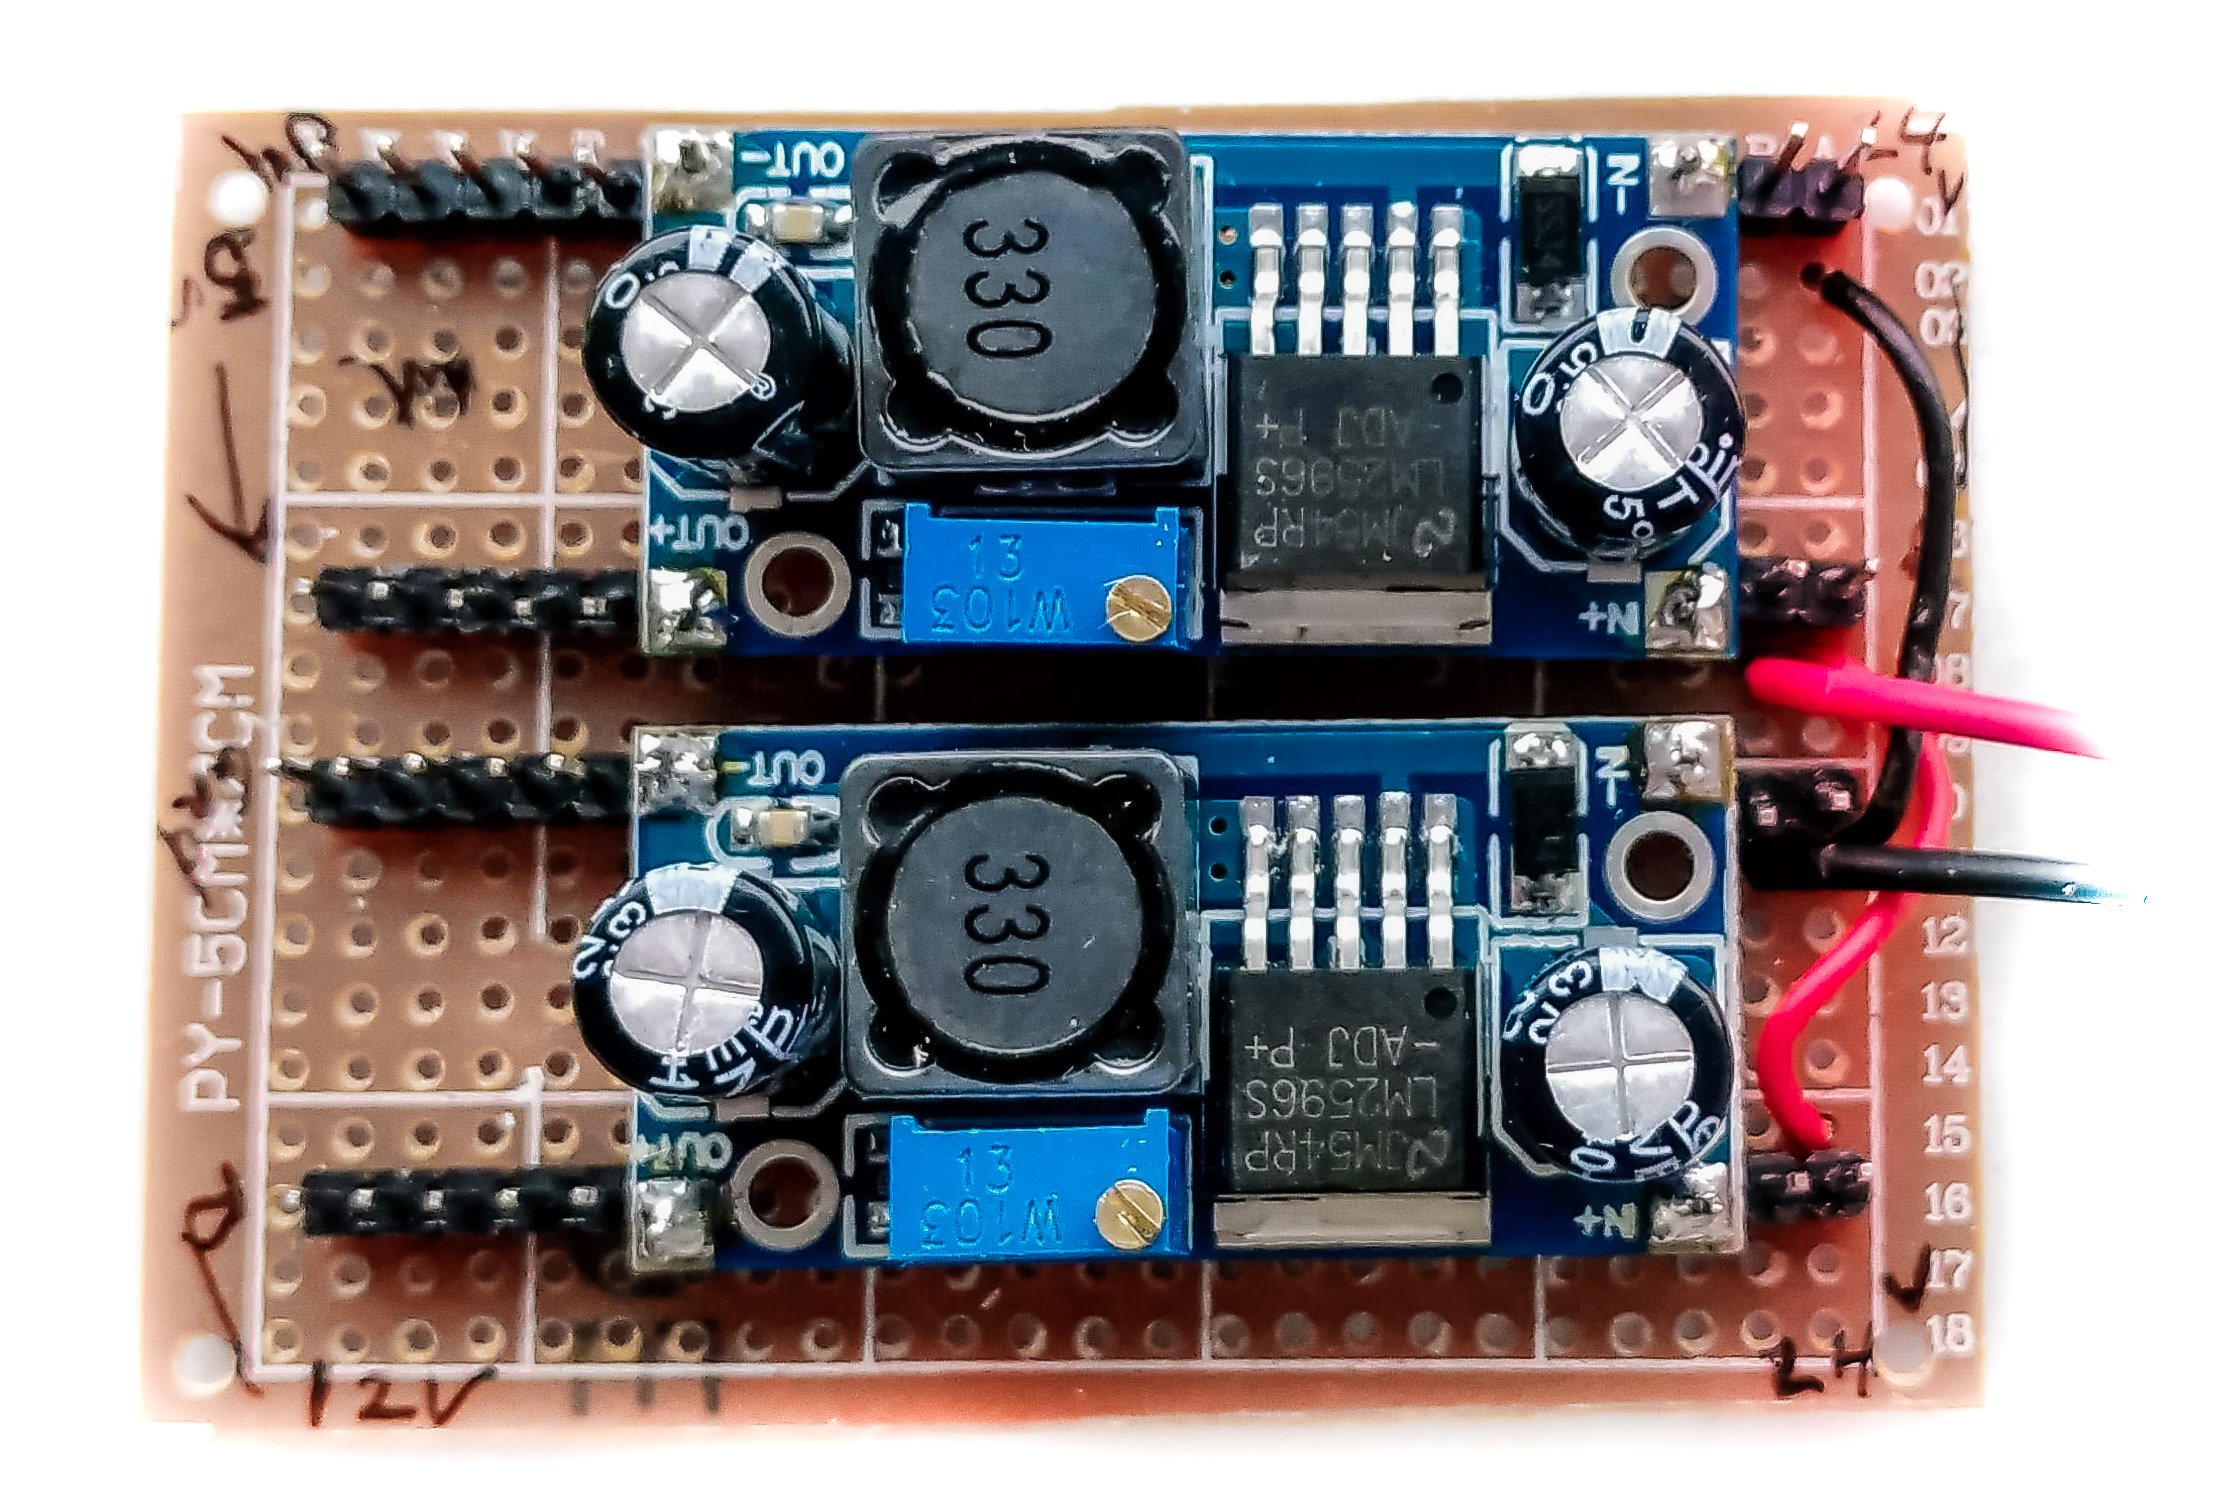
\includegraphics[width=0.42\textwidth]{power_dist}
	\caption{Power distribution board delivering 24V, 12V and 5V to the system.}
	\label{fig:powboard}
\end{figure}

% ================== RGB-LED-COMPONENT =======================
\begin{figure}[h]
	\centering
	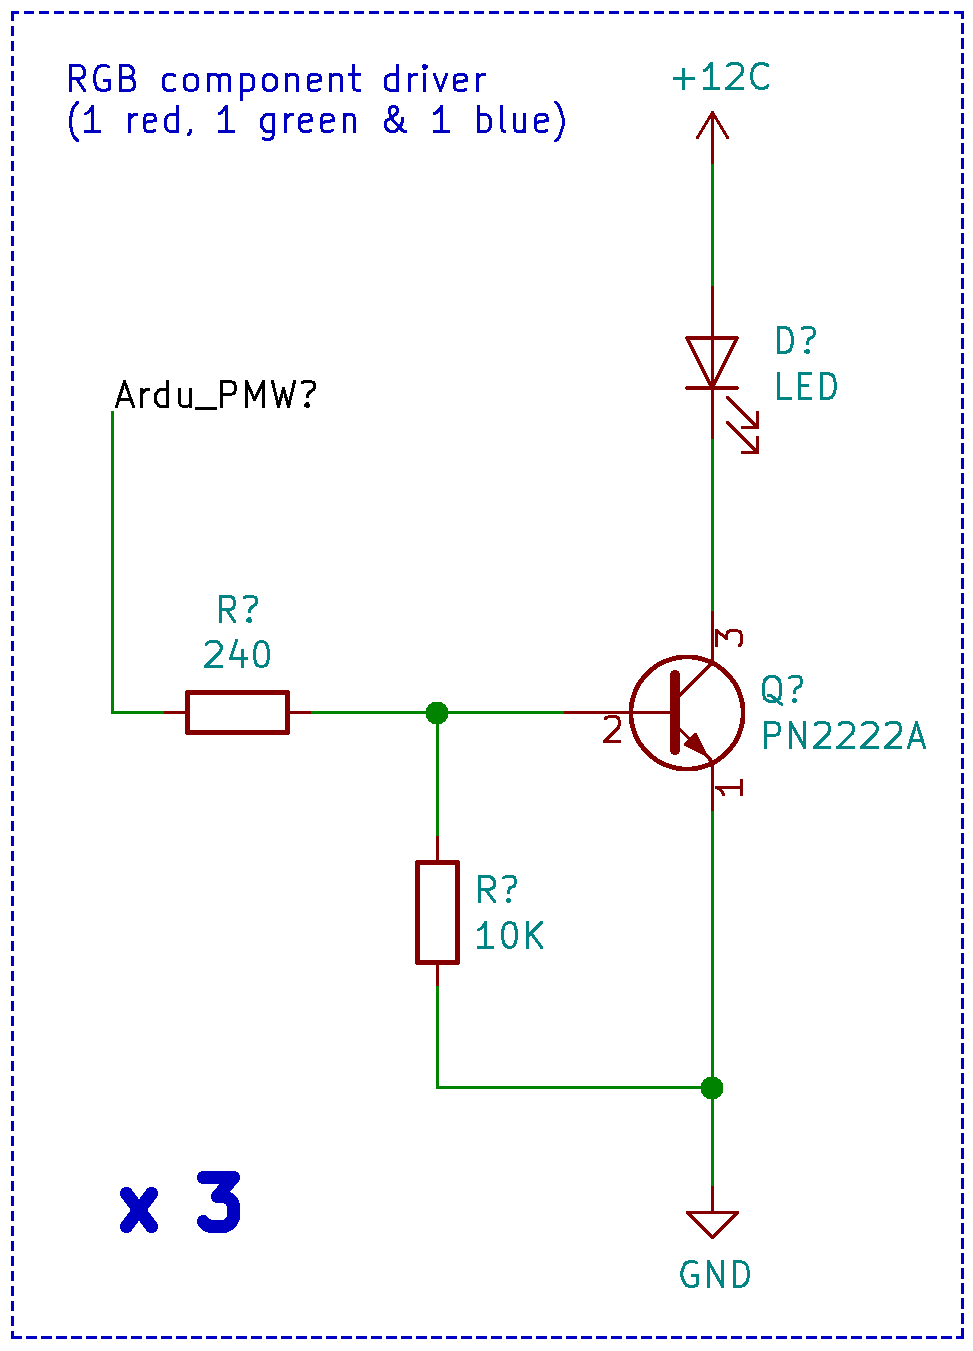
\includegraphics[width=0.38\textwidth]{circuits/rgbled}
	\caption{Schematic of how each color-component of the RGB led strip is driven.}
	\label{cir:rgbled}
\end{figure}

% ================== FLIPPER =======================
\begin{figure*}[h]
	\centering
	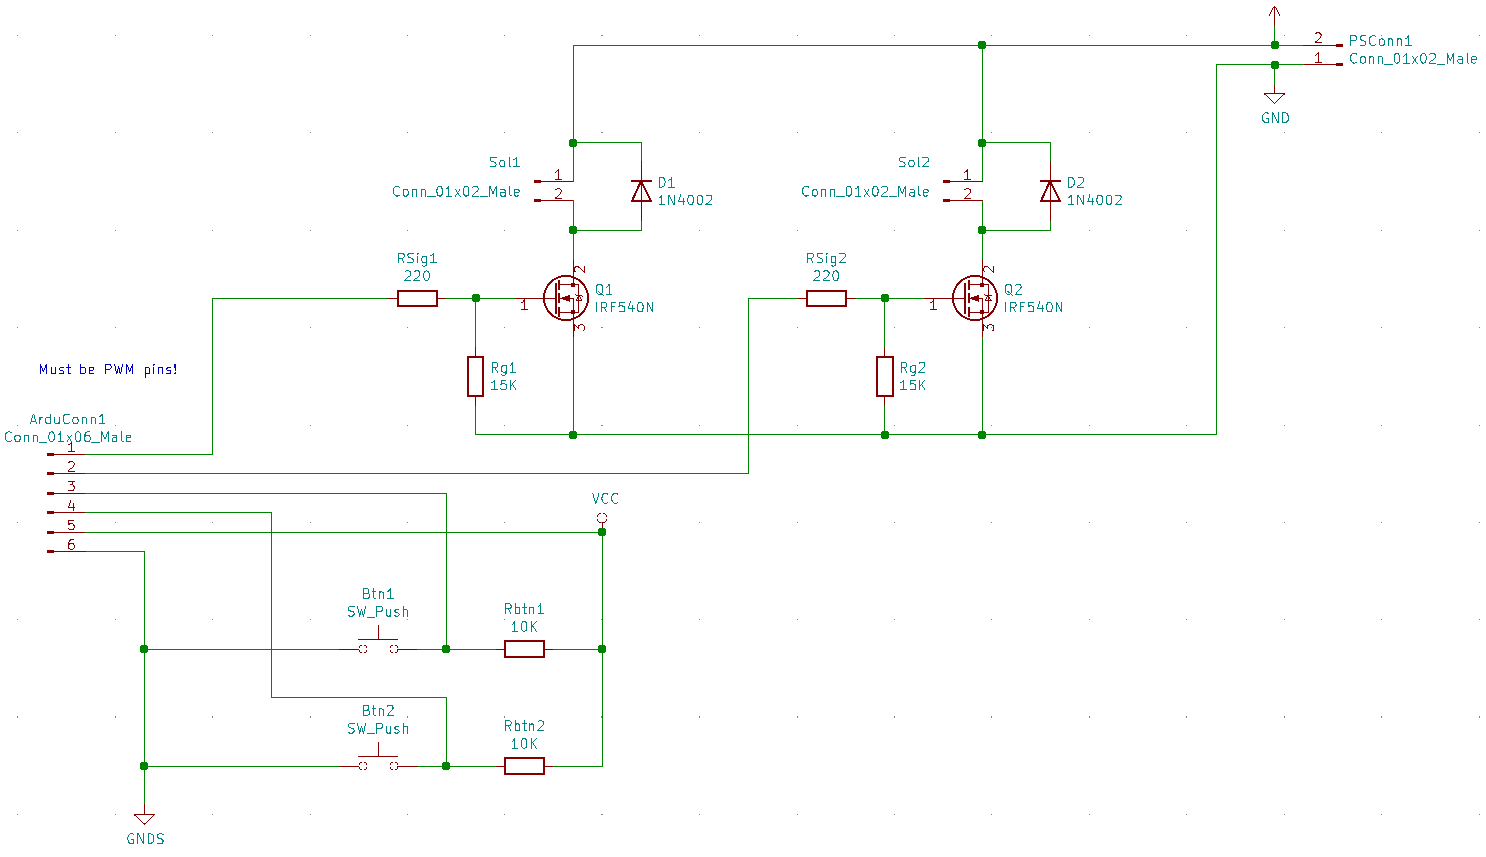
\includegraphics[width=\textwidth]{circuits/flipper}
	\caption{Schematic of the perfboard circuit used to power the flippers.}
	\label{cir:flipper}
\end{figure*}

% ================== BUMPERS =======================
\begin{figure*}[h]
	\centering
	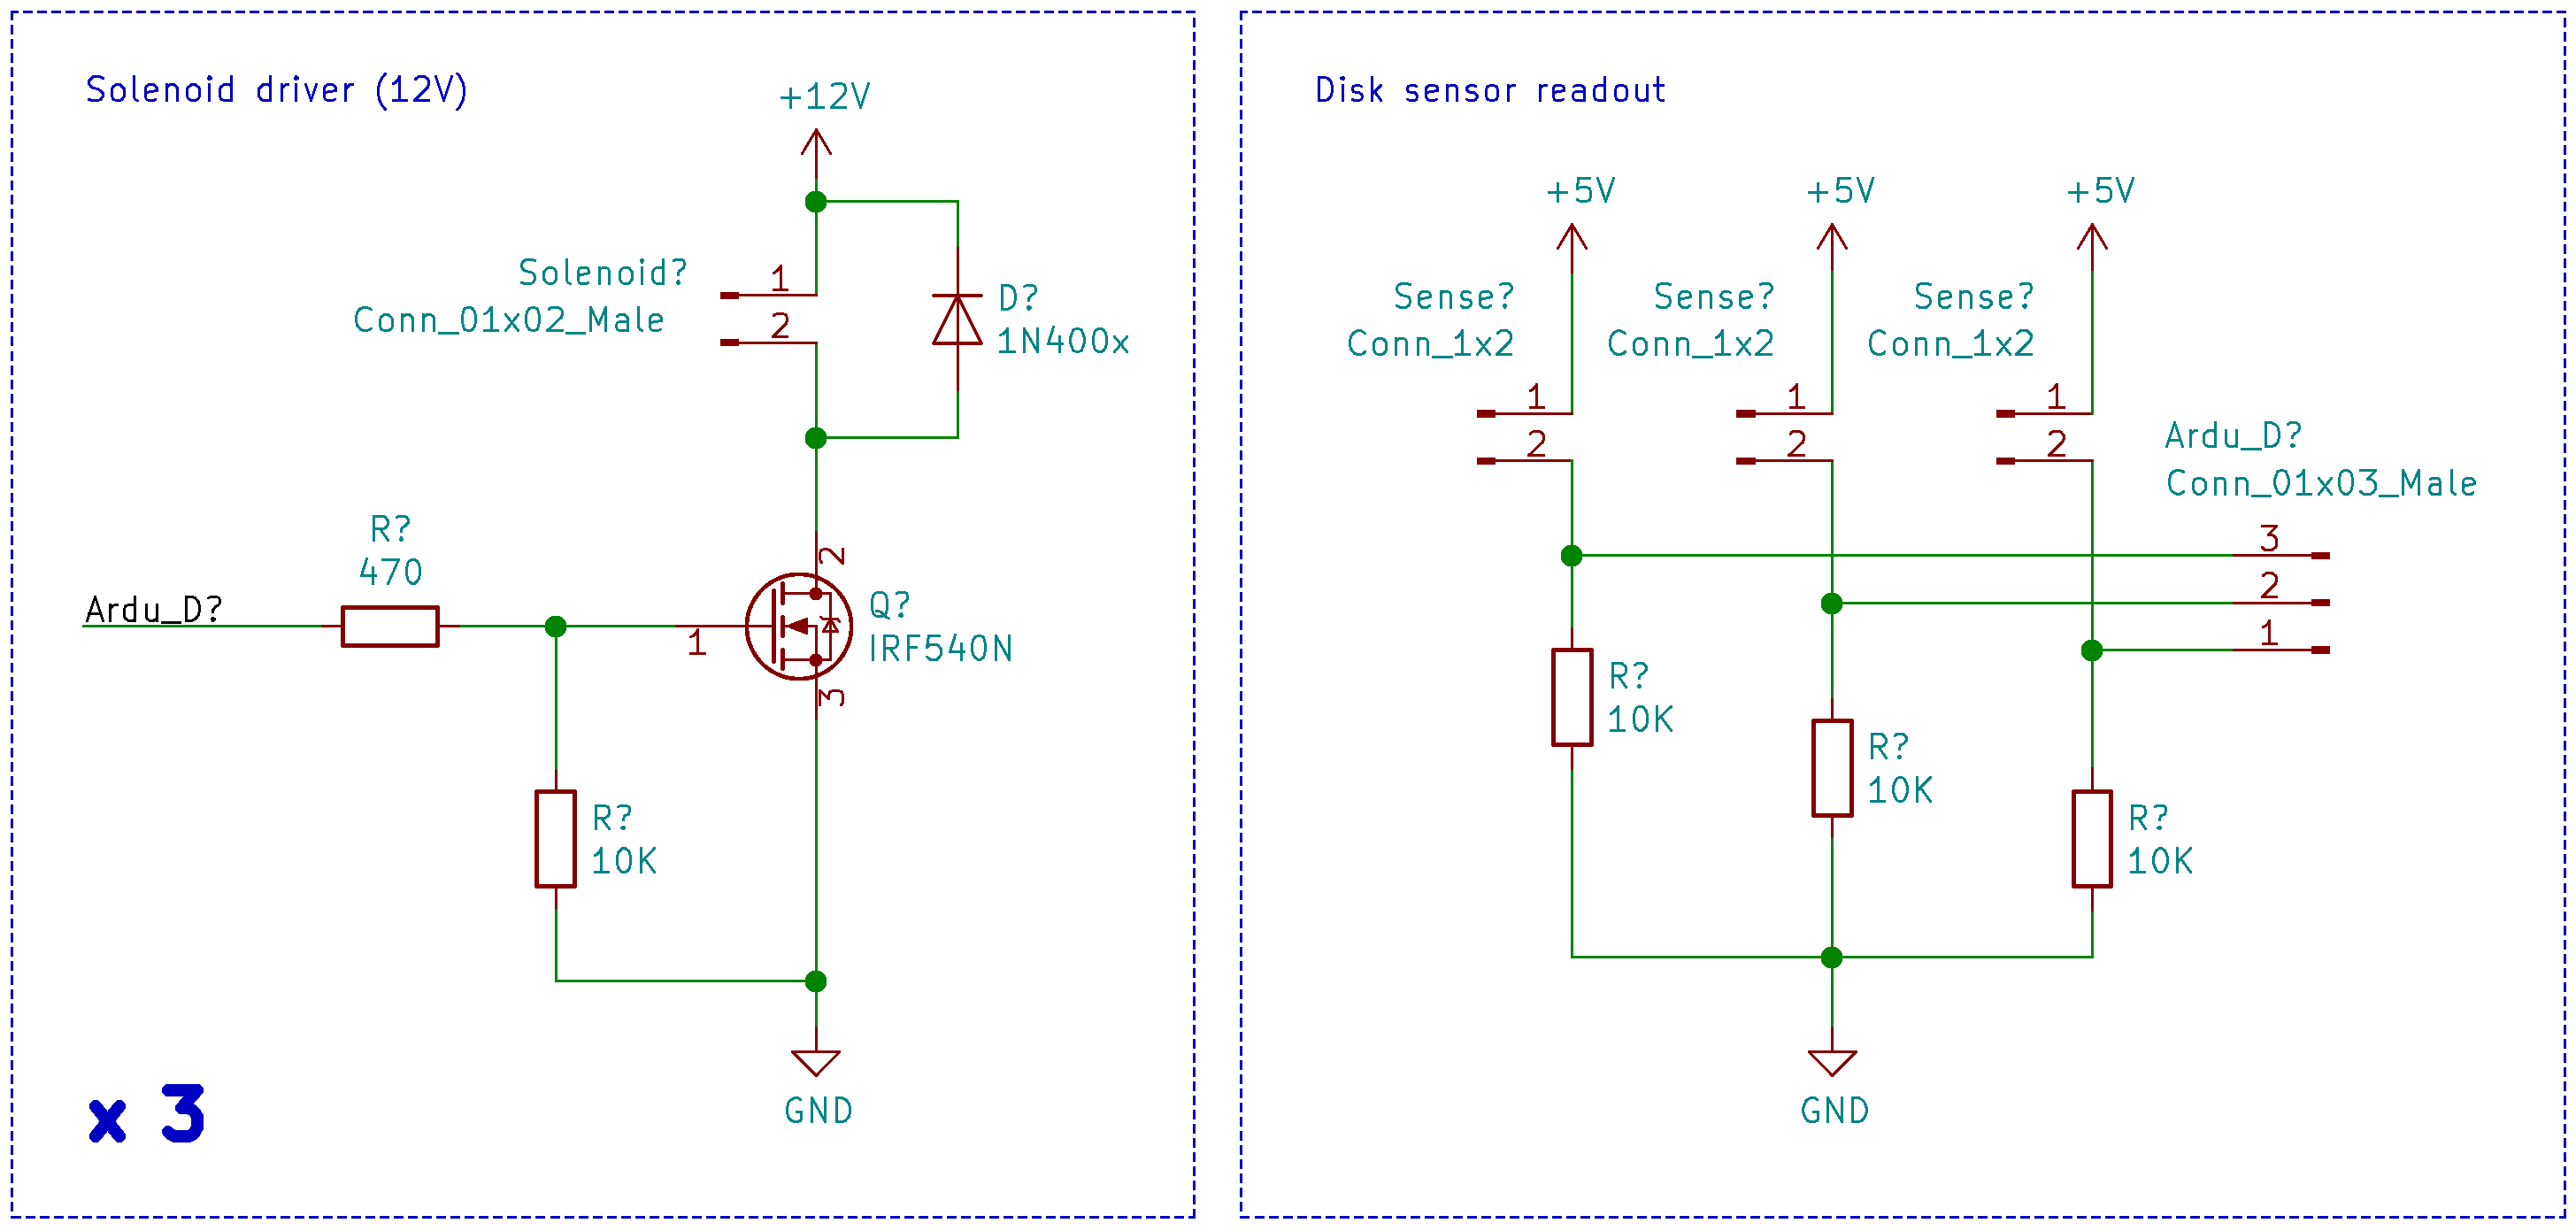
\includegraphics[width=\textwidth]{circuits/popbumper}
	\caption{Schematic of the readout and driver circuit for the pop-bumpers.}
	\label{cir:bumper}
\end{figure*}

% ================== DIVIDERS =======================
\begin{figure*}[h]
	\centering
	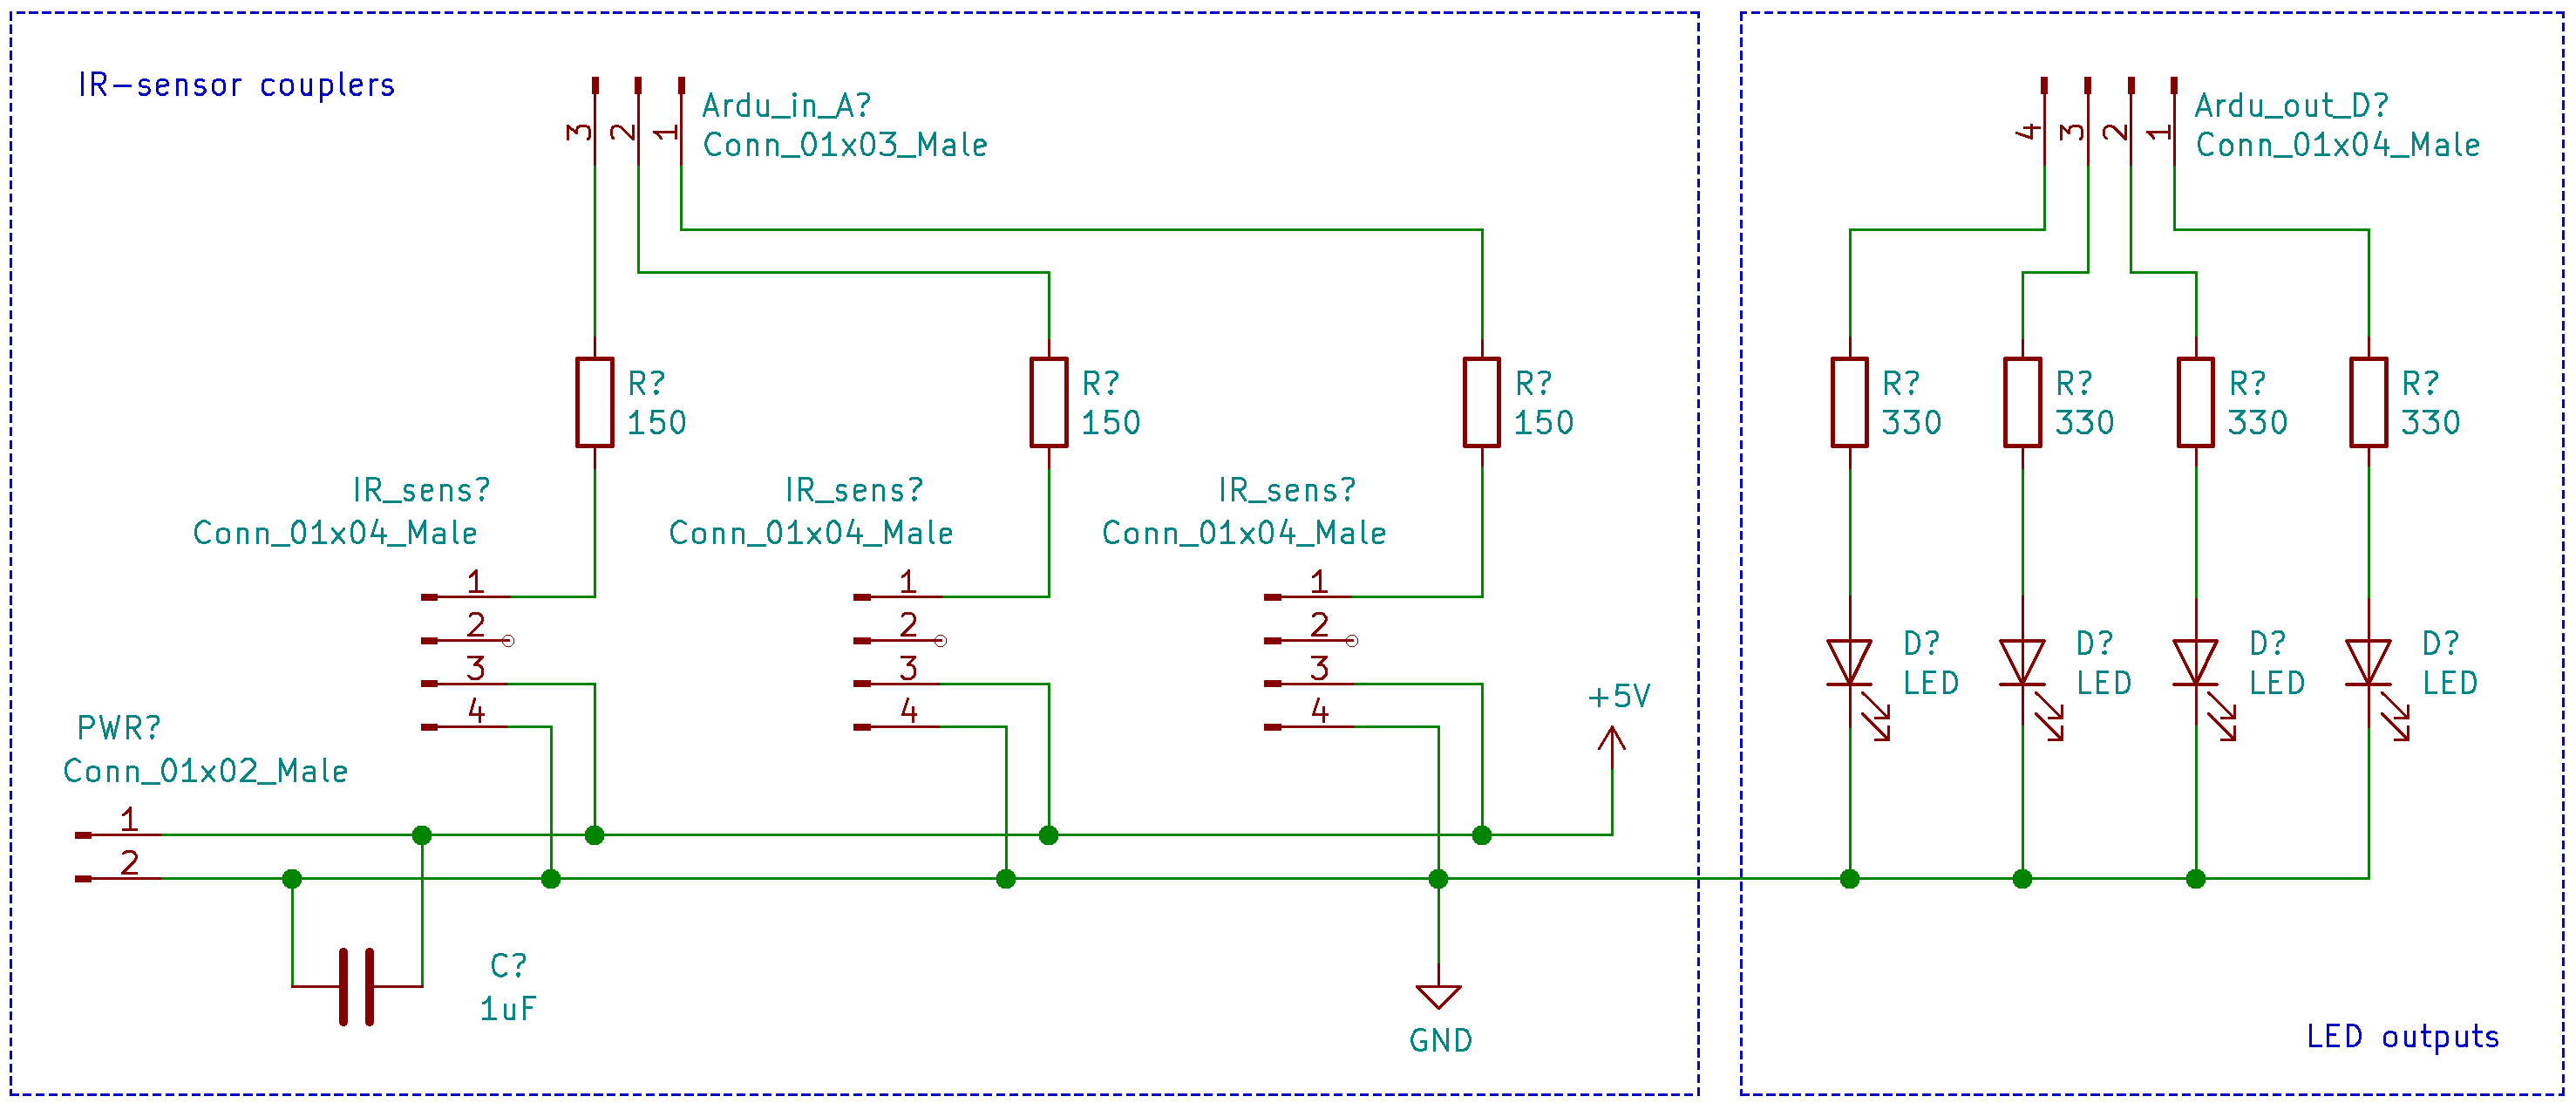
\includegraphics[width=\textwidth]{circuits/toprollers}
	\caption{Schematic of the sensor-coupling and led driver circuit for the top roll-through dividers.}
	\label{cir:top}
\end{figure*}

% ================== LIMIT-SWITCHES =======================
\begin{figure*}[h]
	\centering
	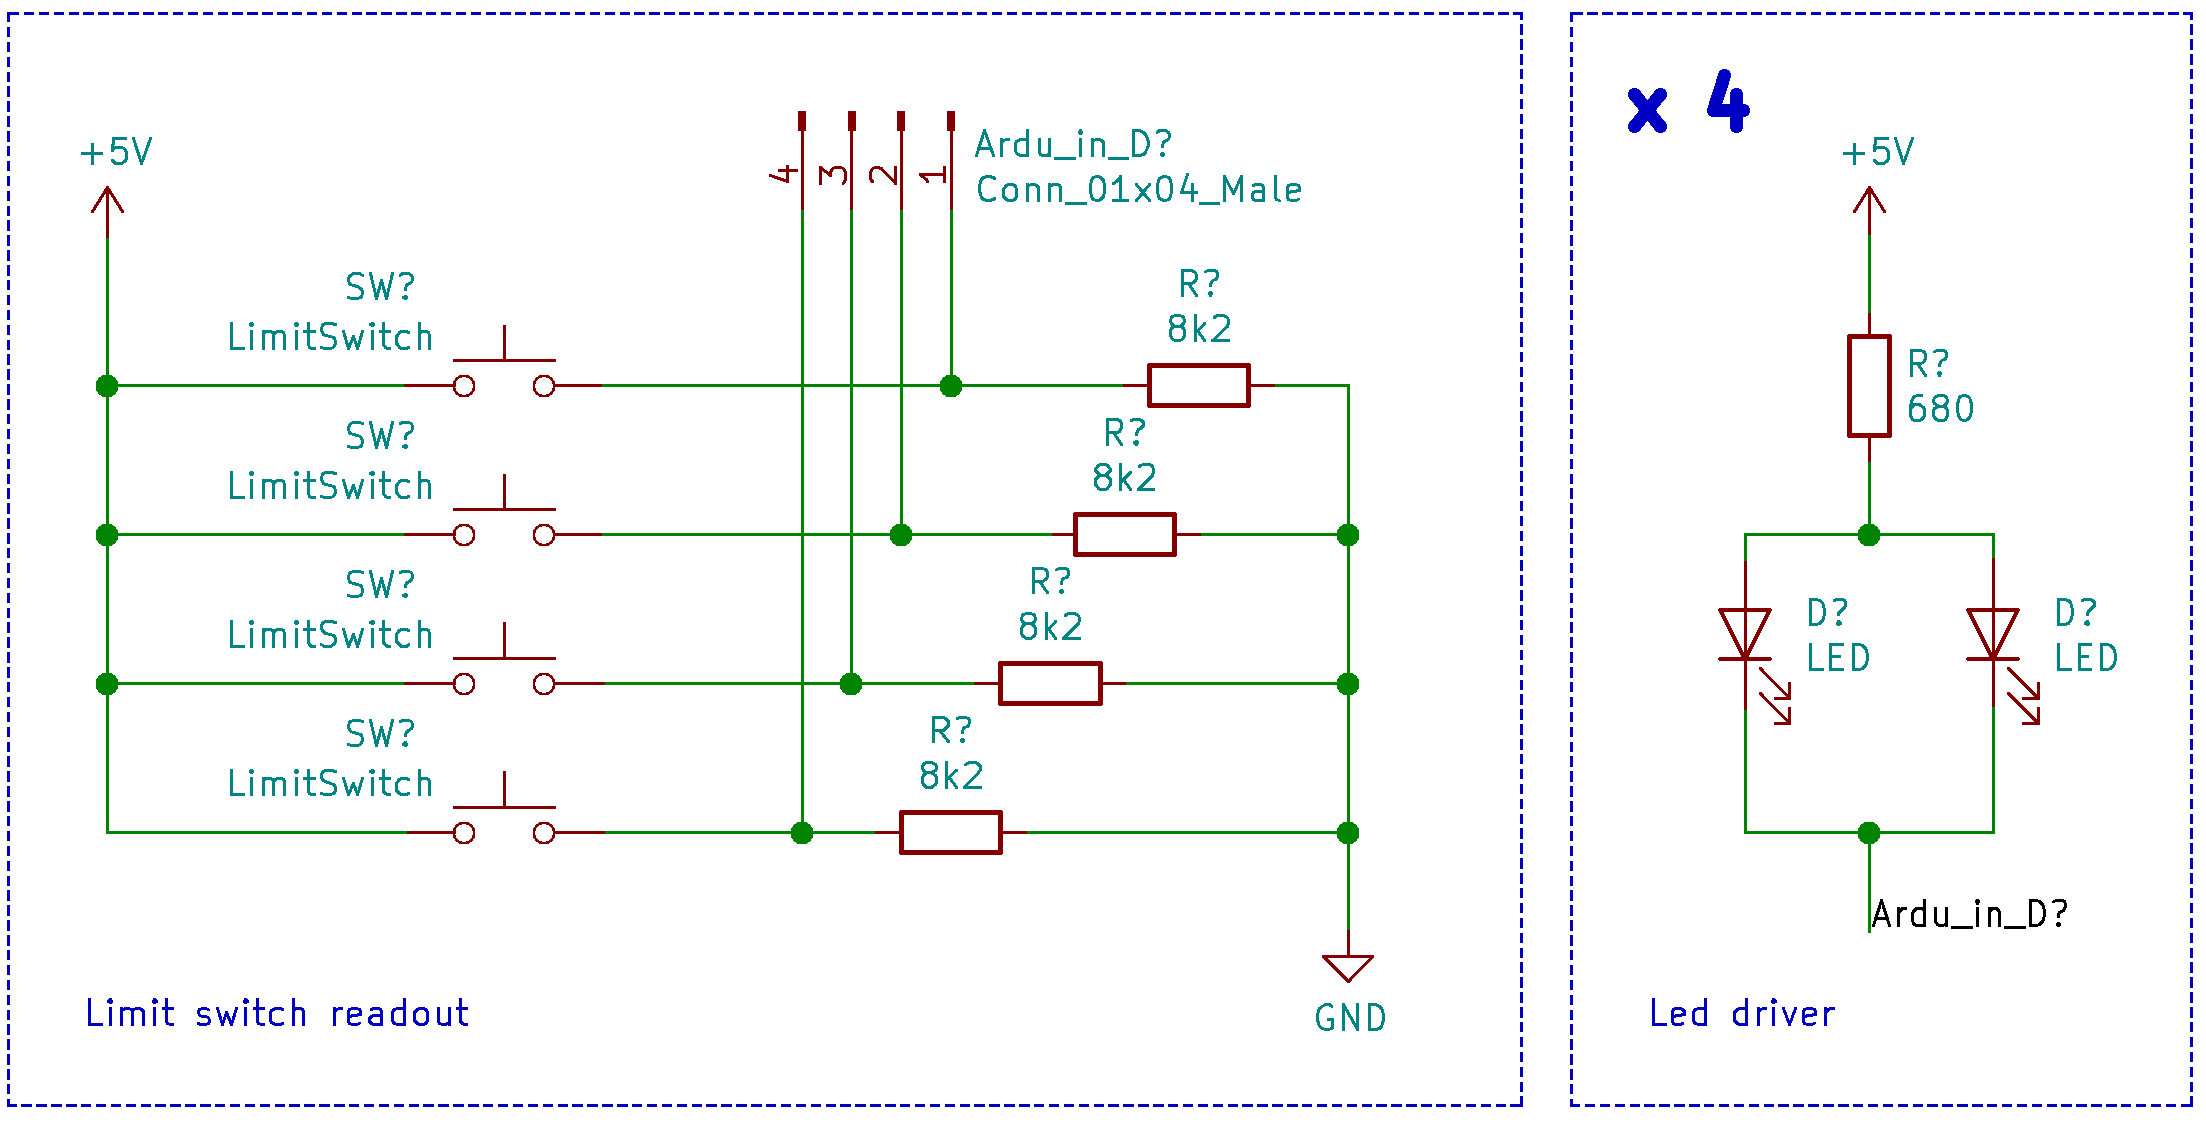
\includegraphics[width=0.8\textwidth]{circuits/limitswitch}
	\caption{Schematic of the limit-switch readout and visual feedback led circuit.}
	\label{cir:switches}
\end{figure*}


\subsection{Software overview}
In this model, each component gets to be a class in its own \verb|.h| (c++) file handling the logic specific for that component in two primary methods; an event polling-method, usually \verb|Read()|, and a time-step method \verb|Update()|. 
The main \verb|.ino| file is responsible for polling each components eventlistener, and calling their appropriate reactive methods (such as activating a pop-bumper, turning an LED on etc.). 
Main repeatedly calls \verb|Update()| in the primary Arduino loop.
In essence, every component becomes a state-machine with \verb|Update()| as its step-function. 
An example snippet from \verb|Main.ino| is shown in \ref{code:main}.
The full structure of the codebase is shown in \ref{fig:codediag}. 

\begin{figure*}
	\begin{lstlisting}[style=c]
  #include "Popbumper.h"
  #include "Flipper.h"
	... // All the subcomponents are brought in here.
	
  // ----- Pin definitions -----
  #define POP1 3      
	... // All used pins are defined here for easy rewiring.
	
  // ----- Global variables -----
  unsigned long score;  // Address passed as argument to each point-giving component
	
  Flipper flipperLeft(BTN_L, FLIP_L);
  Flipper flipperRight(BTN_R, FLIP_R);
  Popbumper bumper1(&score, TAPE1, POP1);
  ... // More imported components are defined here.
	
  // ----- Primary code -----
  void loop() {
		update();
		if(bumper1.IsHit()) { bumper1.Activate(); }
		if(bumper2.IsHit()) { bumper2.Activate(); }
		... // Poll each event-listener function of the subcomponents.
  }
	
  void update() {
 		flipperLeft.Update();
		flipperRight.Update();
		bumper1.Update();
		... // All time-sensitive components are updated at each loop-iteration.
  }
	\end{lstlisting}
	\caption{A snippet of the structure of the main Arduino sketch.}
	\label{code:main}
\end{figure*}


\begin{figure*}[h]
	\centering
	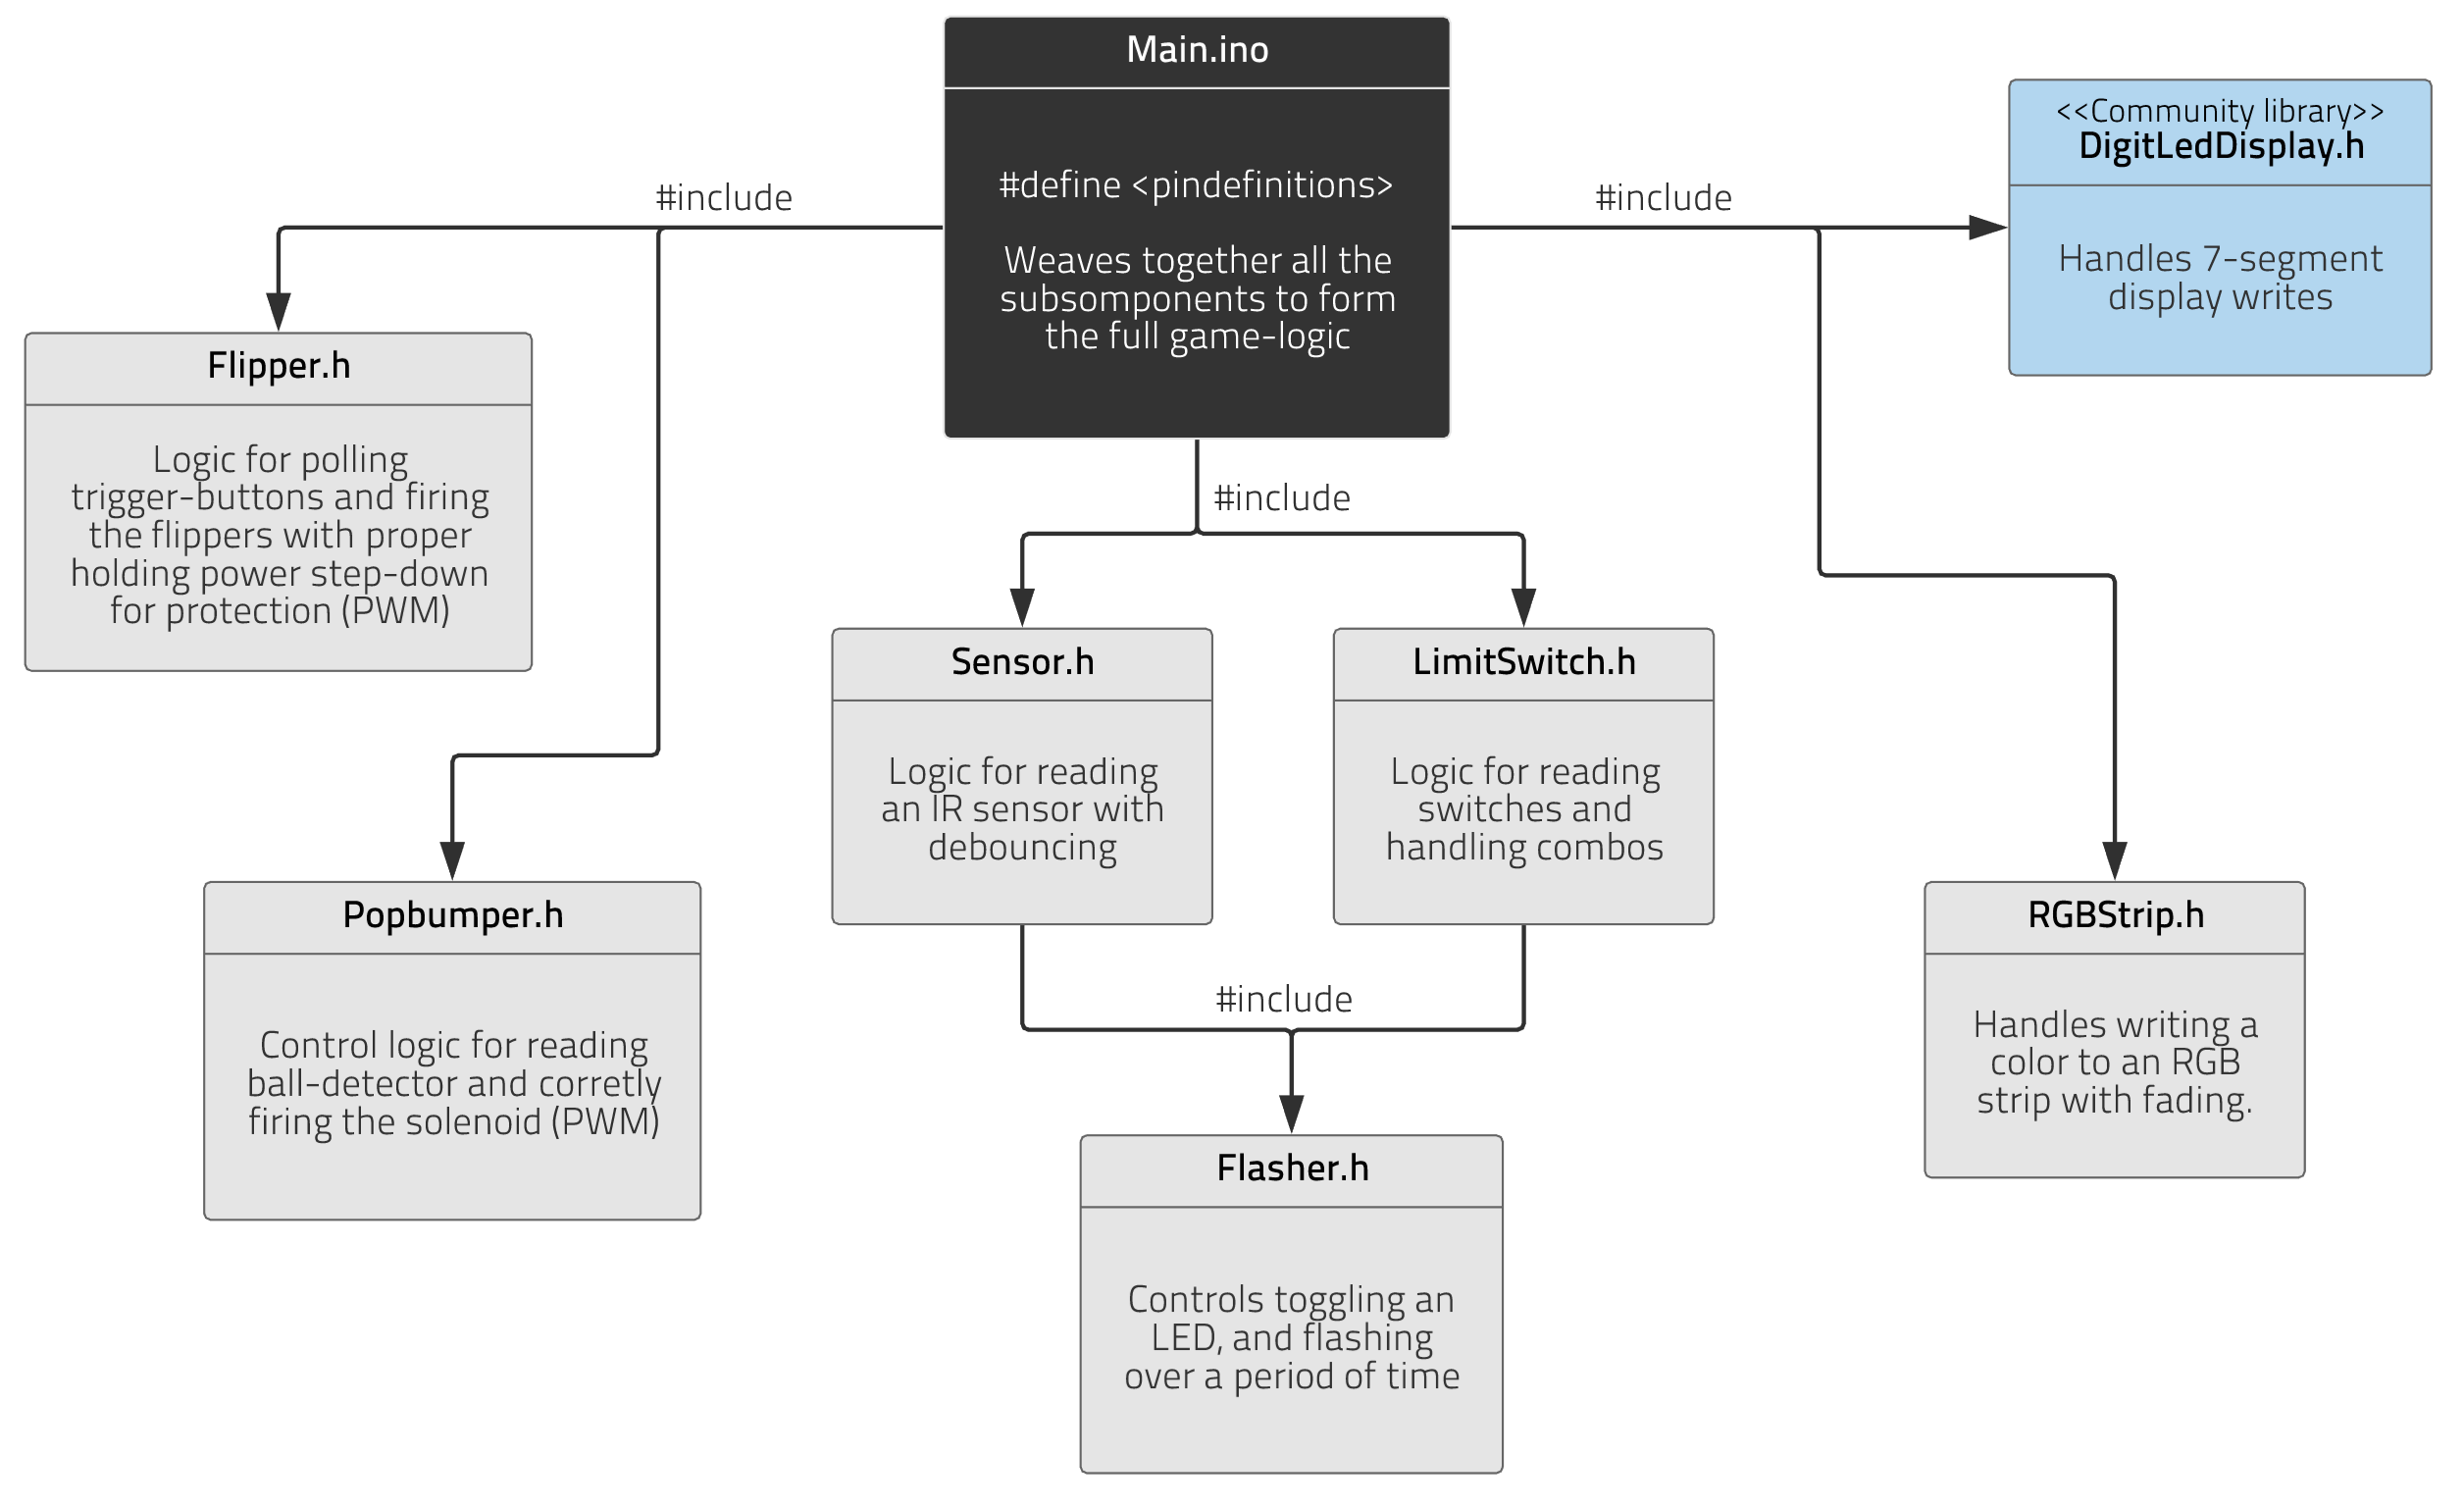
\includegraphics[width=\textwidth]{code_diag}
	\caption{Overview of the code hierarchical structure.}
	\label{fig:codediag}
\end{figure*} \label{appendix:programming model}
\subsection{Laser cutting overview}
\label{appendix:cuts}
This section contains reprensentation of the cuts necessary for the entire machine. See figure \ref{fig:cut01}, \ref{fig:cut02} and \ref{fig:cut03} for these representations. Please see the submitted .PDF files for the actual cutting files appropriate for a laser cutter. 
\begin{figure*}
	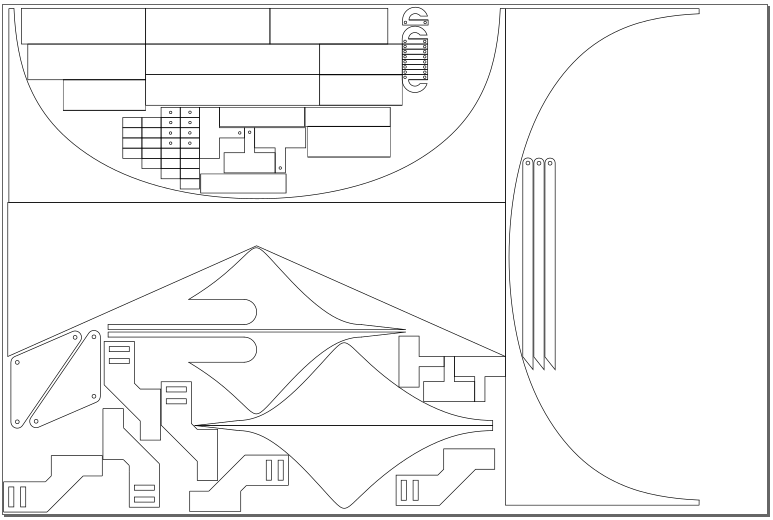
\includegraphics[width=\textwidth]{Cut01}
	\caption{This cut contains brackets and bodywork for the entire machine.}
	\label{fig:cut01}
\end{figure*}
\begin{figure*}
	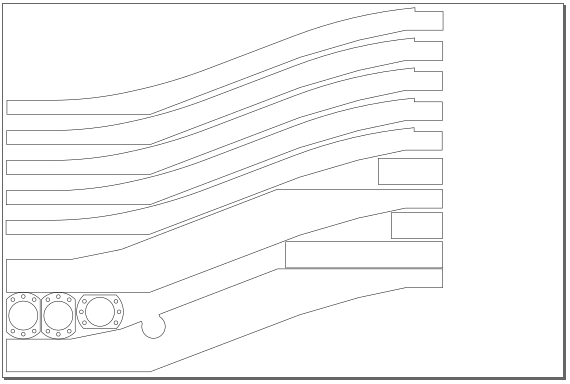
\includegraphics[width=\textwidth]{Cut02}
	\caption{This cut contains the cuts neccessary for the ball-return slide}
	\label{fig:cut02}
\end{figure*}
\begin{figure*}
	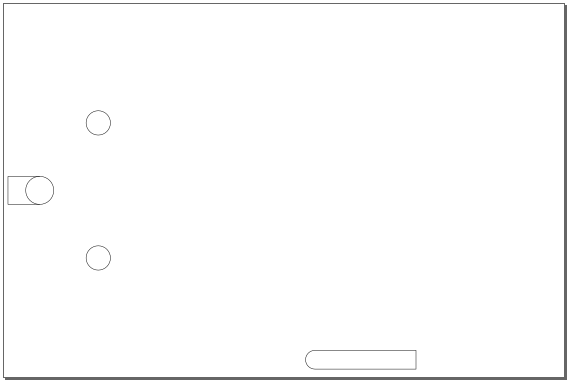
\includegraphics[width=\textwidth]{Cut03}
	\caption{This cut represents the holes neccesary for the playfield. Essentially when cut, the whole board becomes the playfield.}
	\label{fig:cut03}
\end{figure*}

\subsection{BOM}
%TODO: fix scaling
The complete bill of materials is listed in table \ref{tab:bom}, with a supplement of auxiliary components shown in table \ref{tab:bomaux}.

% ====================== Primary ====================================
\begin{table*}[]
\centering
\begin{tabular}{@{}lllll@{}}
\toprule
\textbf{Quantity} & \textbf{Type}  & \textbf{Component}                                   & \textbf{Value / Rating} & \textbf{Used in}                           \\ \midrule
1                 & AC adapter     & 24V Power adapter (230V AC, to 24V DC)               & \textgreater 30W        & Power supply                               \\
2                 & Buck converter & 24V to 5V (\&12V) buck converter (fx. XL6009)        & \textgreater{}= 2A      & Power supply                               \\
2                 & Button         & Large push-button (non-latching)                     &                         & Flippers                                   \\
2                 & Component      & Ball bearing (25mm diameter)                         &                         & Flipper assembly                           \\
1                 & Display        & 7-segment display (MAX7219 8-bit digital controlled) &                         & Points display                             \\
2                 & LED-strip      & 0.5m RGB LED-strip (fx 5050 SMD's)                   & 12V (\textless 1A)      & Lighting                                   \\
3                 & Material       & Sheet (600 x 400 x 4mm) (MDF or Acrylic)             &                         & Complete laser cutting                     \\
4                 & Material       & Spring                                               &                         & Ball launcher, Self-closing door, Flippers \\
3                 & Material       & Elastic band                                         &                         & Pop bumpers                                \\
1                 & Material       & Tubing                                               &                         & Ball return mechanism                      \\
2                 & Material       & Bendable metal rods (50mm diameter)                  &                         & Ramp                                       \\
4                 & Material       & Plywood (15 x 600 x 400mm)                           &                         & Outer box                                  \\
5                 & MosFET         & IRF540N Mosfet (N-channel)                           & \textgreater{}2A @ 24V  & Flippers, Popbumpers                       \\
4                 & Sensor         & IR sensor (4-pin, w. LM393 controller)               &                         & Dividers, Falldown detector                \\
3                 & Solenoid       & Linear Solenoid                                      & 12V                     & Pop bumpers                                \\
2                 & Solenoid       & Linear Solenoid                                      & 24V/12V                 & Flippers                                   \\
4                 & Switch         & Low-resistance end limit-switch                      & 5V                      & Switch targets                             \\
3                 & Transistor     & PN2222 High-current transistor                       & \textgreater{}1A @ 12V  & Lighting                                   \\ \bottomrule
\end{tabular}
\caption{Bill of materials}
\label{tab:bom}
\end{table*}

% ========================== Auxiliary ====================== 
\begin{table*}[]
	\centering
	\begin{tabular}{@{}llll@{}}
		\toprule
		\textbf{Type} & \textbf{Component}                              & \textbf{Value / Rating} & \textbf{Used in}        \\ \midrule
		Nuts \& bolts & Various sizes, most around 2 \&3 mm in diameter &                         & Mounting                \\
		Resistor      & Through-hole resistor                           & 1/4W                    & Various circuits        \\
		LED           & 5 \& 3.5 mm LEDs, assortment of colours         & 5V                      & Lighting and decoration \\
		Diode         & Kick-back absorbing diodes, fx. 1N4001          & \textgreater{}= 1A      & Flippers, Popbumpers    \\ \bottomrule
	\end{tabular}
	\caption{Auxiliary components (Quantity not specified)}
	\label{tab:bomaux}
\end{table*}

\end{document}